\documentclass[10pt]{beamer}

\usetheme{metropolis}
\usepackage{appendixnumberbeamer}

\usepackage{algorithm}
\usepackage{algpseudocode}
\usepackage{amsfonts}
\usepackage[ngerman]{babel}
\usepackage{booktabs}
\usepackage[scale=2]{ccicons}
\usepackage{graphicx}
\usepackage{hyperref}
\usepackage{lipsum}
\usepackage{listings}
\usepackage{multirow}
\usepackage{pgfplots}
\usepackage{xcolor}

\usepgfplotslibrary{dateplot}

\usepackage{xspace}
\newcommand{\themename}{\textbf{\textsc{metropolis}}\xspace}

\addto{\captionsngerman}{%
  \renewcommand*{\figurename}{Abb.}
}

\let\svthefootnote\thefootnote

\definecolor{mGreen}{rgb}{0,0.6,0}
\definecolor{mGray}{rgb}{0.5,0.5,0.5}
\definecolor{mPurple}{rgb}{0.58,0,0.82}

\lstdefinestyle{CStyle}{
    commentstyle=\color{mGreen},
    keywordstyle=\color{magenta},
    numberstyle=\tiny\color{mGray},
    stringstyle=\color{mPurple},
    basicstyle=\footnotesize,
    breakatwhitespace=false,
    breaklines=true,
    captionpos=b,
    keepspaces=true,
    numbers=left,
    numbersep=5pt,
    showspaces=false,
    showstringspaces=false,
    showtabs=false,
    tabsize=2,
    language=C
}

\title{Ein skalierbarer Löser für Randwertprobleme unter Verwendung der
       Greenschen Kreuzapproximationsmethode und GPUs}
\date{\today}
\author{Bennet Carstensen}
\institute{Christian-Albrechts-Universität zu Kiel\\
           Institut für Informatik\\
           Scientific Computing}
% \titlegraphic{\hfill\includegraphics[height=1.5cm]{logo.pdf}}

\begin{document}

\maketitle

\begin{frame}{Agenda}
  \setbeamertemplate{section in toc}[sections numbered]
  \tableofcontents[hideallsubsections]
\end{frame}

\section{Einleitung}

\begin{frame}{Randwertprobleme}
  \begin{columns}
    \column{0.575\linewidth}
      \begin{itemize}
        \visible<1->{\item Wird verwendet in der
                     \begin{itemize}
                       \item Elektrostatik
                       \item Wärmeleitung
                       \item Akustik
                     \end{itemize}}
        \item \visible<1->{Sei \(\Omega \subseteq \mathbb{R}^{d}\) gegeben,
                           \(d \in \{ 2, 3 \}\)}
        \item \visible<2->{\(\int\limits_{\Omega} g(x, y) u(y) dy = f(x)
                           \text{ für alle } x \in \Omega\)}
      \end{itemize}
    \column{0.33\linewidth}
      \centering
      \begin{overprint}
        \onslide<1>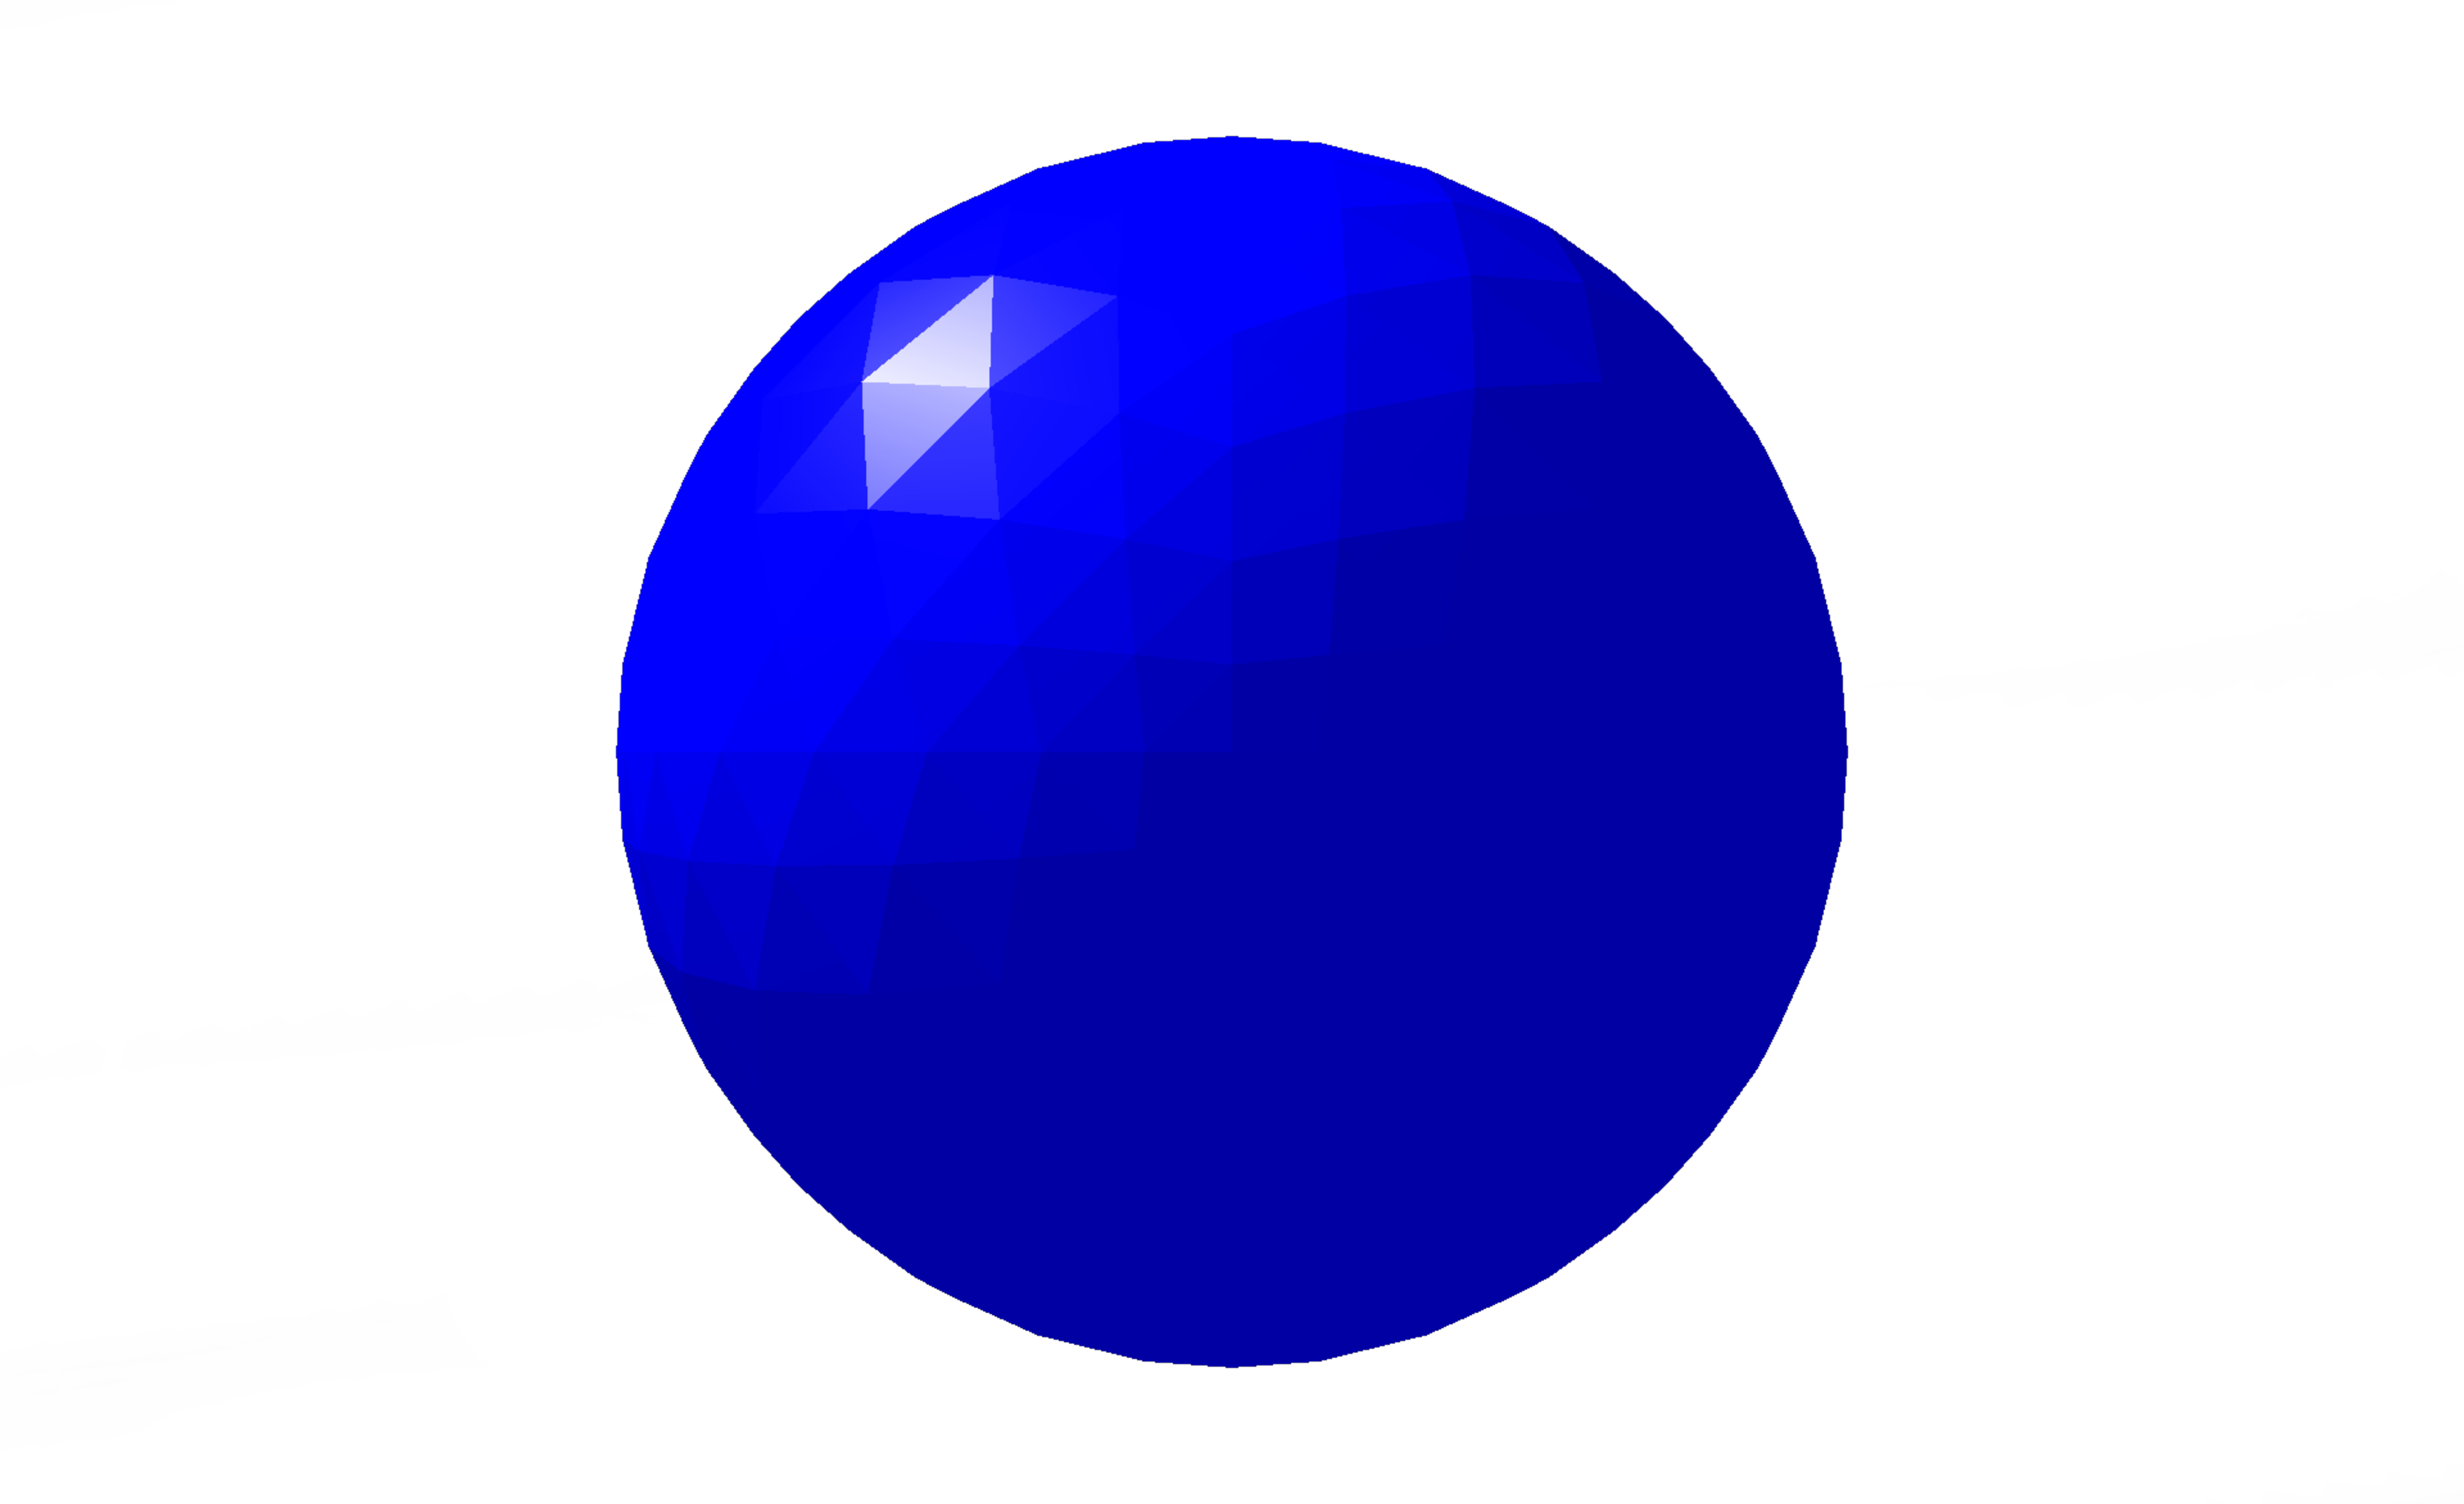
\includegraphics[width=1.5\linewidth]{figures/fg-sphere-full.pdf}
        \onslide<2>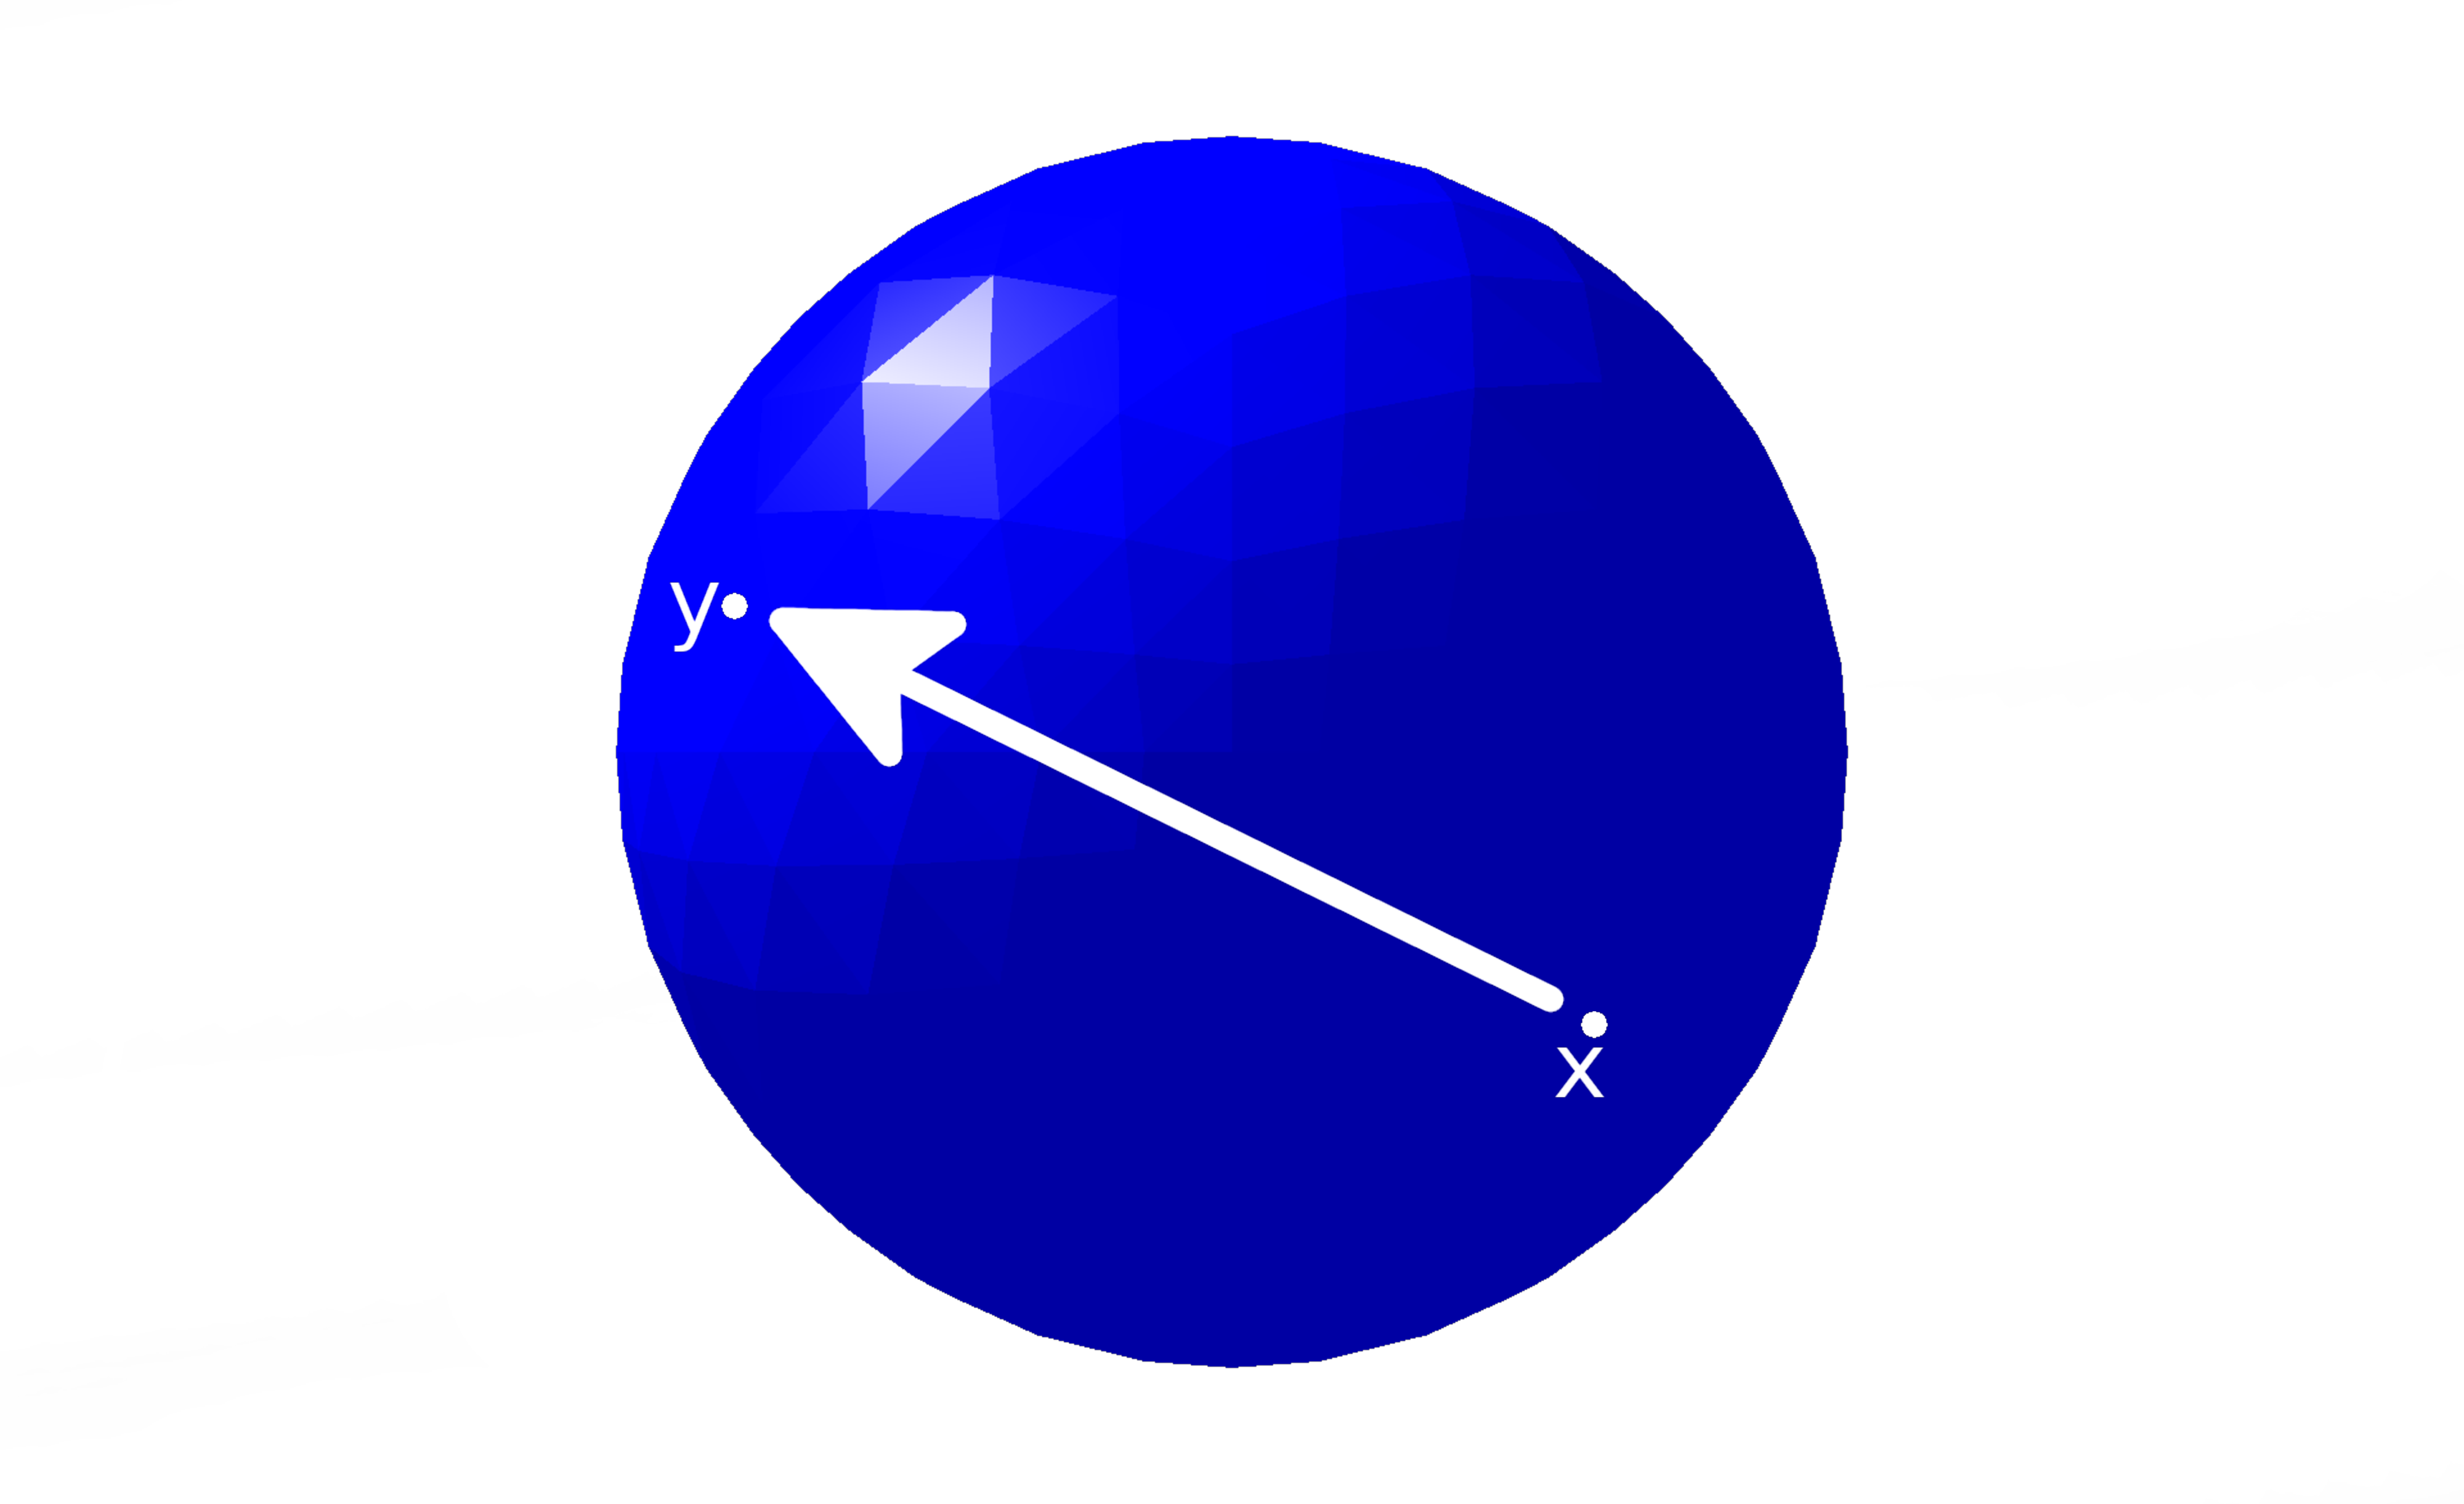
\includegraphics[width=1.5\linewidth]{figures/fg-sphere-full-inf.pdf}
      \end{overprint}

  \end{columns}
  \footnotesize
  \let\thefootnote\relax\footnote{Quelle: \href{https://link.springer.com/article/10.1007\%2Fs00211-015-0757-y}{Approximation of integral operators by Green quadrature and nested cross approximation.}}
  \addtocounter{footnote}{-1}\let\thefootnote\svthefootnote\relax
  \normalsize
\end{frame}

\begin{frame}{Diskretisierung}
  \begin{columns}
    \column{0.575\linewidth}
      Diskretisierung durch Basisfunktionen\\
      \({(\varphi_{i})}_{i = 1}^{n} \text{ und }
        {(\psi_{j})}_{j = 1}^{n}, n \in \mathbb{N}\)
      \begin{itemize}
        \item \(V_{n} = span\{ \varphi_{i} : i \in \{ 1, \hdots, n\}\}, \newline
               U_{n} = span\{ \psi_{j} : j \in \{ 1, \hdots, n\}\}\)
        \item Finde \(u_{n} \in U_{n}\) mit\\
        \(\int\limits_{\Omega} v_{n}(x) \int\limits_{\Omega} g(x,y) \
        u_{n}(y) \ dy \ dx = \int\limits_{\Omega} v_{n}(x) \ f(x) \ dx\)\\
        für alle \(v_{n} \in V_{n}\)
      \end{itemize}
    \column{0.33\linewidth}
      \centering
      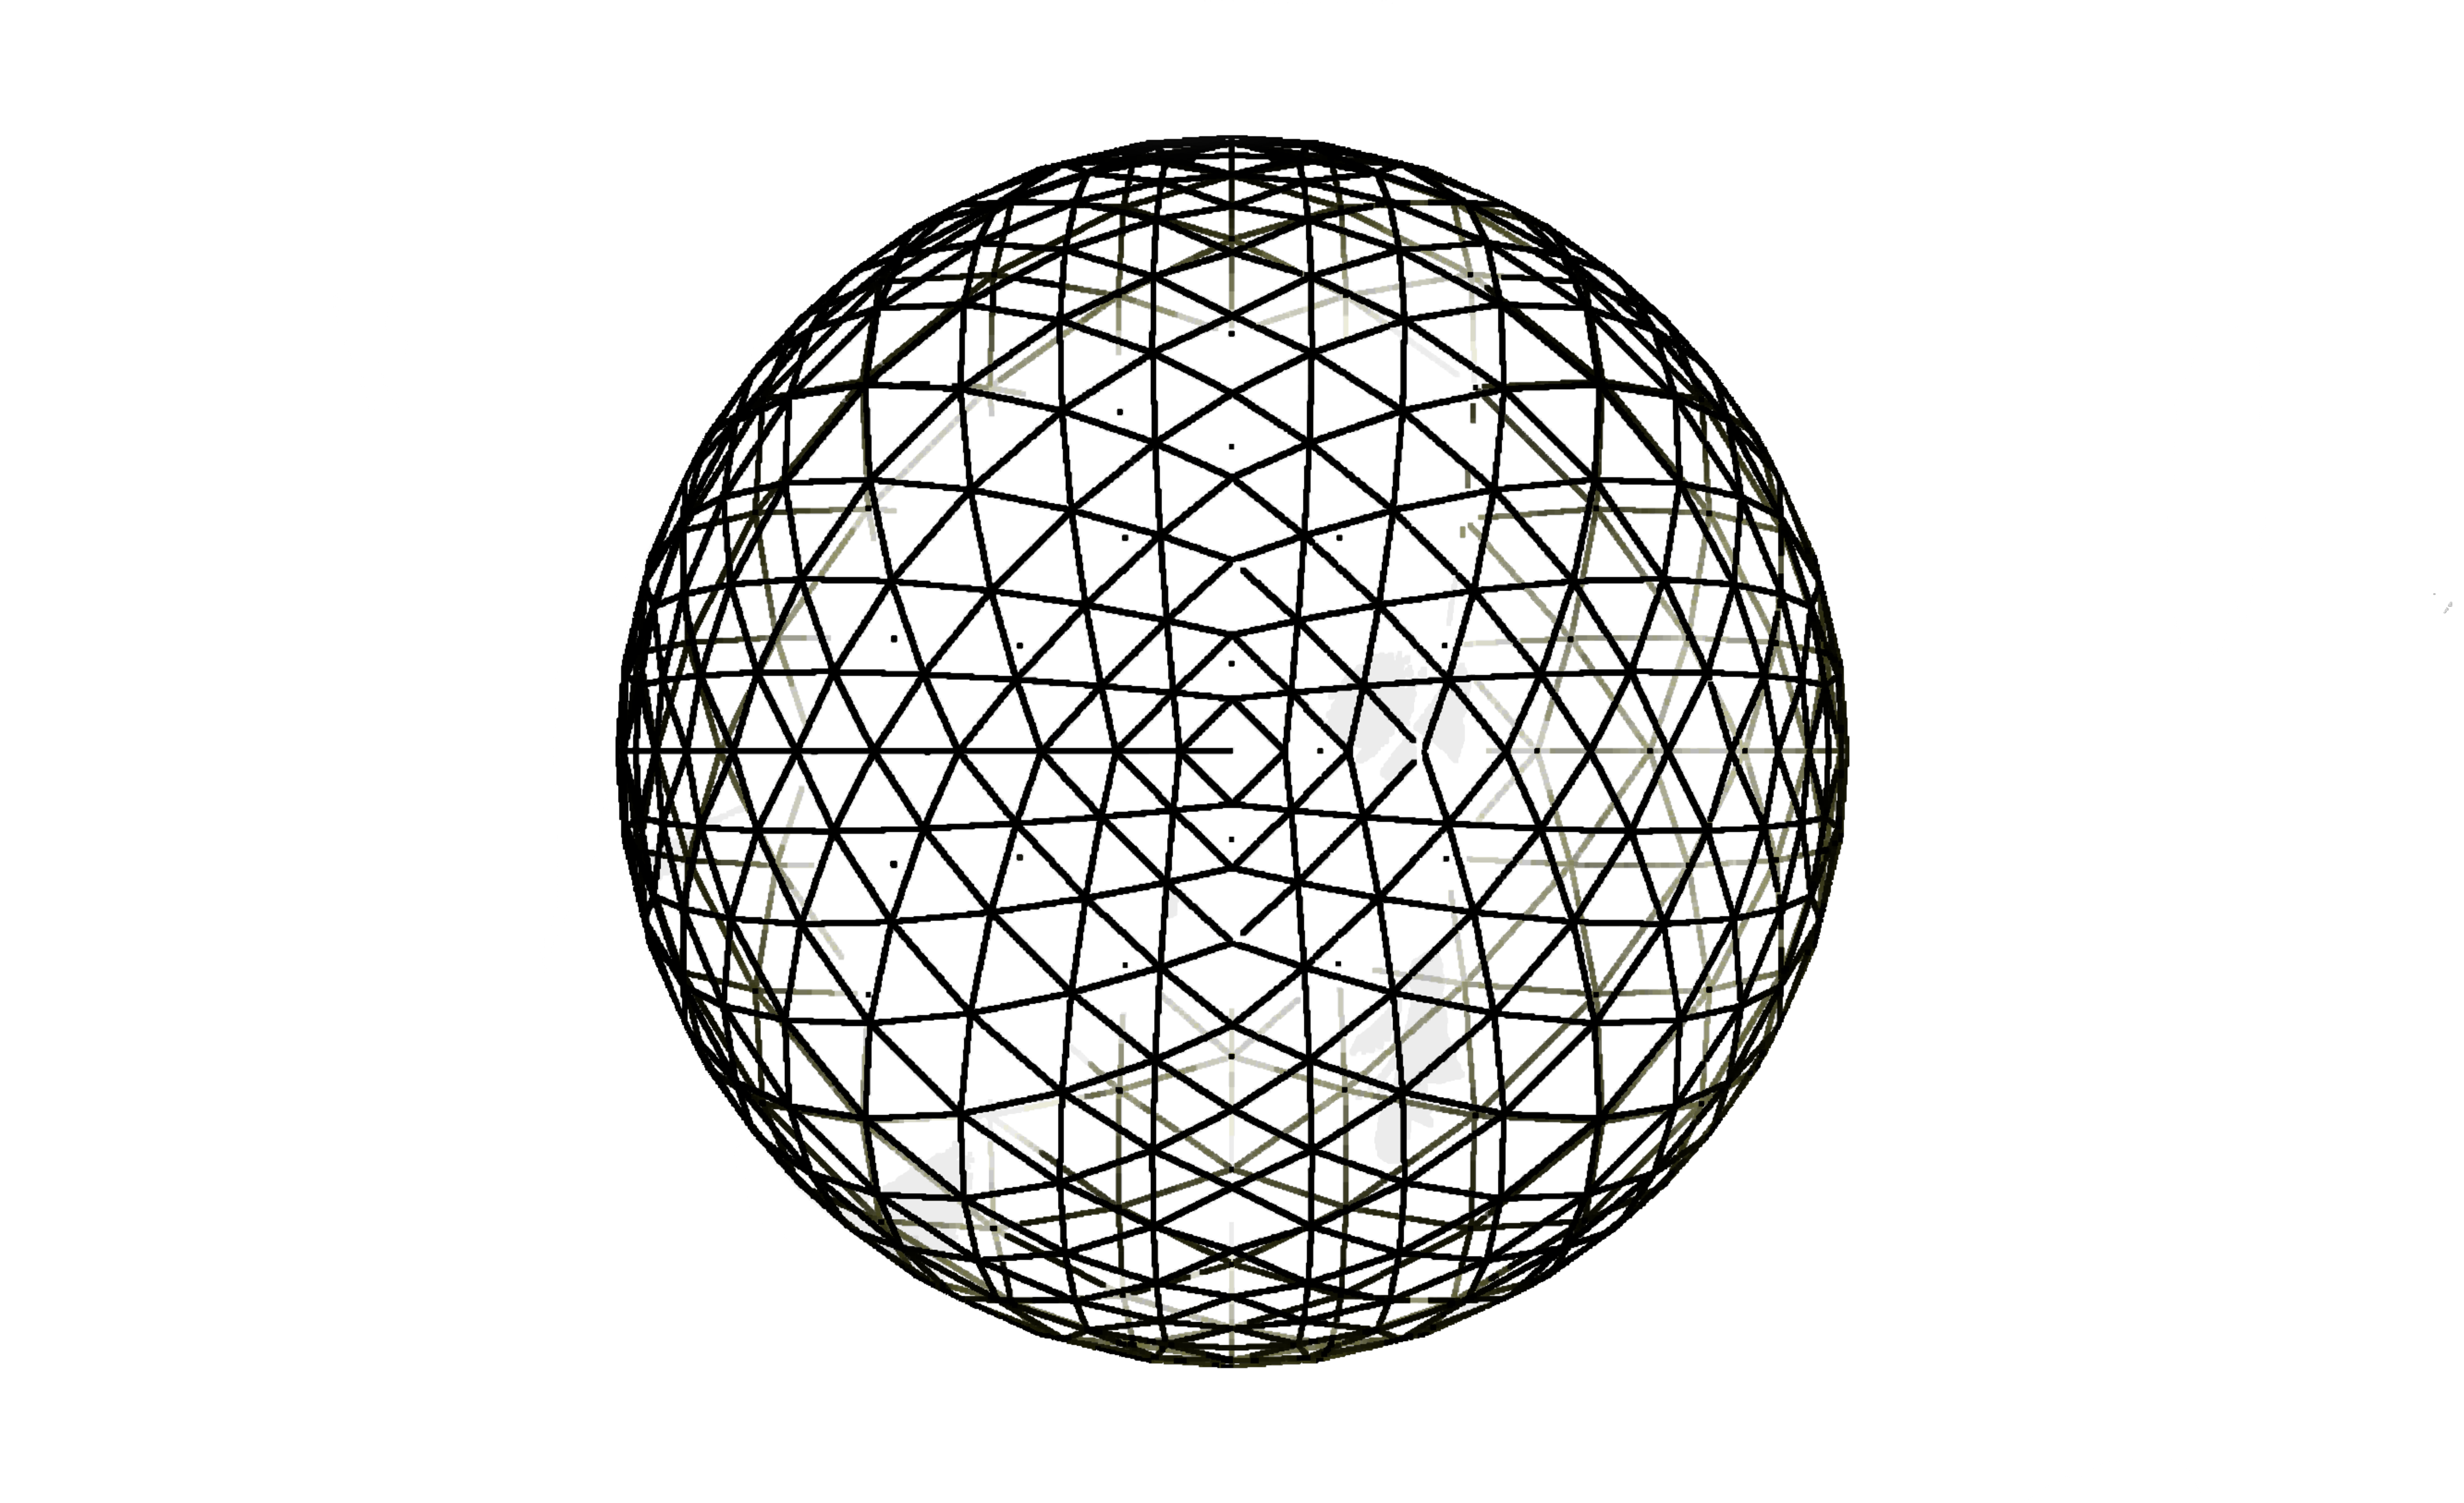
\includegraphics[width=1.5\linewidth]{figures/fg-sphere-tri.pdf}
  \end{columns}
  \footnotesize
  \let\thefootnote\relax\footnote{Quelle: \href{https://link.springer.com/article/10.1007\%2Fs00211-015-0757-y}{Approximation of integral operators by Green quadrature and nested cross approximation.}}
  \addtocounter{footnote}{-1}\let\thefootnote\svthefootnote\relax
  \normalsize
\end{frame}

\begin{frame}{Lineares Gleichungssystem}
  Sei \(u_{n}  = \sum\limits_{j = 1}^{n} \varphi_{j} z_{j}, z_{j} \in
        \mathbb{R} \)
  \begin{itemize}
    \item Finde \(z = (z_{1}, \hdots, z_{n}) \in \mathbb{R}^{n}\) mit\\
          \(Gz = b\)
    \item \(g_{ij} = \int\limits_{\Omega} \varphi_{i}(x) \int\limits_{\Omega}
            g(x, y) \ \psi_{j}(y) \ dy \ dx\)
    \item \(b_{i} = \int\limits_{\Omega} \varphi_{i} \ f(x) \ dx\)
    \item \(i, j \in \{ 1, \hdots, n \}\)
  \end{itemize}
  \footnotesize
  \let\thefootnote\relax\footnote{Quelle: \href{https://link.springer.com/article/10.1007\%2Fs00211-015-0757-y}{Approximation of integral operators by Green quadrature and nested cross approximation.}}
  \addtocounter{footnote}{-1}\let\thefootnote\svthefootnote\relax
  \normalsize
\end{frame}

\begin{frame}{Probleme \& Lösungsansätze}
  \begin{overprint}
    \onslide<1-2>
      \begin{table}[h]
        \begin{tabular}{ccc} \toprule
                    & \multicolumn{2}{c}{Speicherbedarf (in GB)} \\
          Dimension & Galerkin & \\ \midrule
              16384 &      1.0 & \\
              32768 &      4.0 & \\
              65536 &     16.0 & \\
             131072 &     64.0 & \\
             262144 &    256.0 & \\ \bottomrule
        \end{tabular}
      \end{table}
    \onslide<3>
      \begin{table}[h]
        \begin{tabular}{ccc} \toprule
                    & \multicolumn{2}{c}{Speicherbedarf (in GB)} \\
          Dimension & Galerkin & \(\mathcal{H}^2\)-Matrix \\ \midrule
              16384 &      1.0 & 0.20613 \\
              32768 &      4.0 & 0.43834 \\
              65536 &     16.0 & 0.88314 \\
             131072 &     64.0 & 1.80900 \\
             262144 &    256.0 & 3.57143 \\ \bottomrule
        \end{tabular}
      \end{table}
  \end{overprint}

  \begin{itemize}
    \item \visible<1->{Problem: \(G\) meist vollbesetzt \(\Rightarrow\) hohe
                       Speicheranforderungen und Rechenaufwand}
    \visible<2->{\item Lösungsansätze:}
    \begin{itemize}
      \item \visible<2->{Schnelle Multipol-Methode (bessere
                         Laufzeitkomplexität)}
      \item \visible<3->{\(\mathcal{H}^2\)-Matrizen +
                           Greensche Kreuzapproximationsmethode\\
                           (engl. \textit{Green cross approximation (GCA)
                           method})\\
                           (geringere Speicheranforderungen \(\Rightarrow\)
                           bessere Laufzeitkomplexität)}
    \end{itemize}
  \end{itemize}
\end{frame}

\begin{frame}{Problem \& Lösungsansätze}
  \begin{figure}
    \centering
    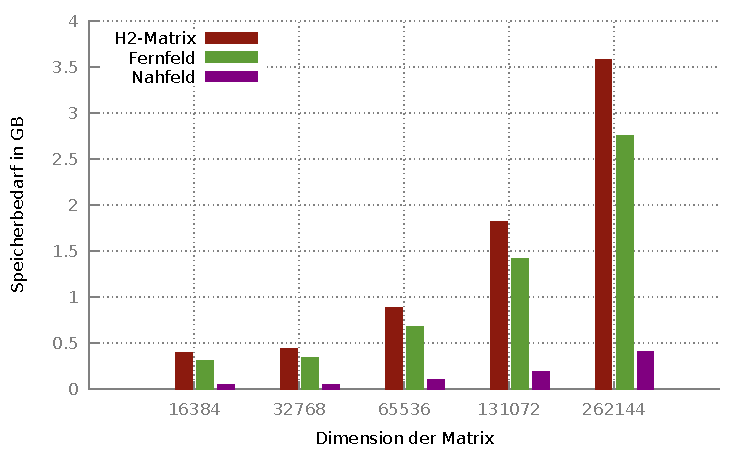
\includegraphics[width=.45\linewidth]{figures/fg-memory-h2-nf-ff.pdf}
    \caption{Speicherbedarf einer \(\mathcal{H}^2\)-Matrix und deren Blockmatrizen.}

  \end{figure}
  \begin{itemize}
    \item Problem: Reale Problemstellungen benötigen immer größere Matrizen
          \(\Rightarrow\) reduzierte Speicheranforderungen durch
          \(\mathcal{H}^2\)-Matrizen haben ihre Grenzen
    \item Lösungsansätz:
    \begin{itemize}
      \item Mehr Arbeitsspeicher
      \item Berechne reproduzierbare Untermatrizen einer
            \(\mathcal{H}^2\)-Matrix on-the-fly, wenn sie benötigt werden.
            (75-90 \% des Speicherbedarfs wird eingespart)
    \end{itemize}
  \end{itemize}
\end{frame}

\begin{frame}{Problem \& Lösungsansätze}
  \begin{table}[h]
    \begin{tabular}{ccc} \toprule
                & \multicolumn{2}{c}{Performanz in ms} \\
      Dimension & \(\mathcal{H}^2\)-MVM & \(\mathcal{H}^2\)-MVM + Blockmatrizen on-the-fly \\ \midrule
          16384 &                66.239 &   50985.5 \\
          32768 &               149.201 &  109092 \\
          65536 &               227.471 &  220589 \\
         131072 &               476.539 &  451777 \\ \bottomrule
    \end{tabular}
  \end{table}
  \begin{itemize}
    \item Problem: Wesentlich größerer Rechenaufwand bei letzterem Ansatz
    \item Lösungsansatz (diese Masterarbeit):
    \begin{itemize}
      \item Quadratur zur Auswertung der Integrale bestimmt Performance
      \item Quadratur ist äußerst parallelisierbar/vektorisierbar
      \item Auslagern der Auswertungen auf eine Grafikkarte
    \end{itemize}
  \end{itemize}
\end{frame}

\section{\(\mathcal{H}^2\)-Matrizen}

\begin{frame}{\(\mathcal{H}^2\)-Matrizen}
  \begin{figure}
    \begin{overprint}
      \onslide<1>\centering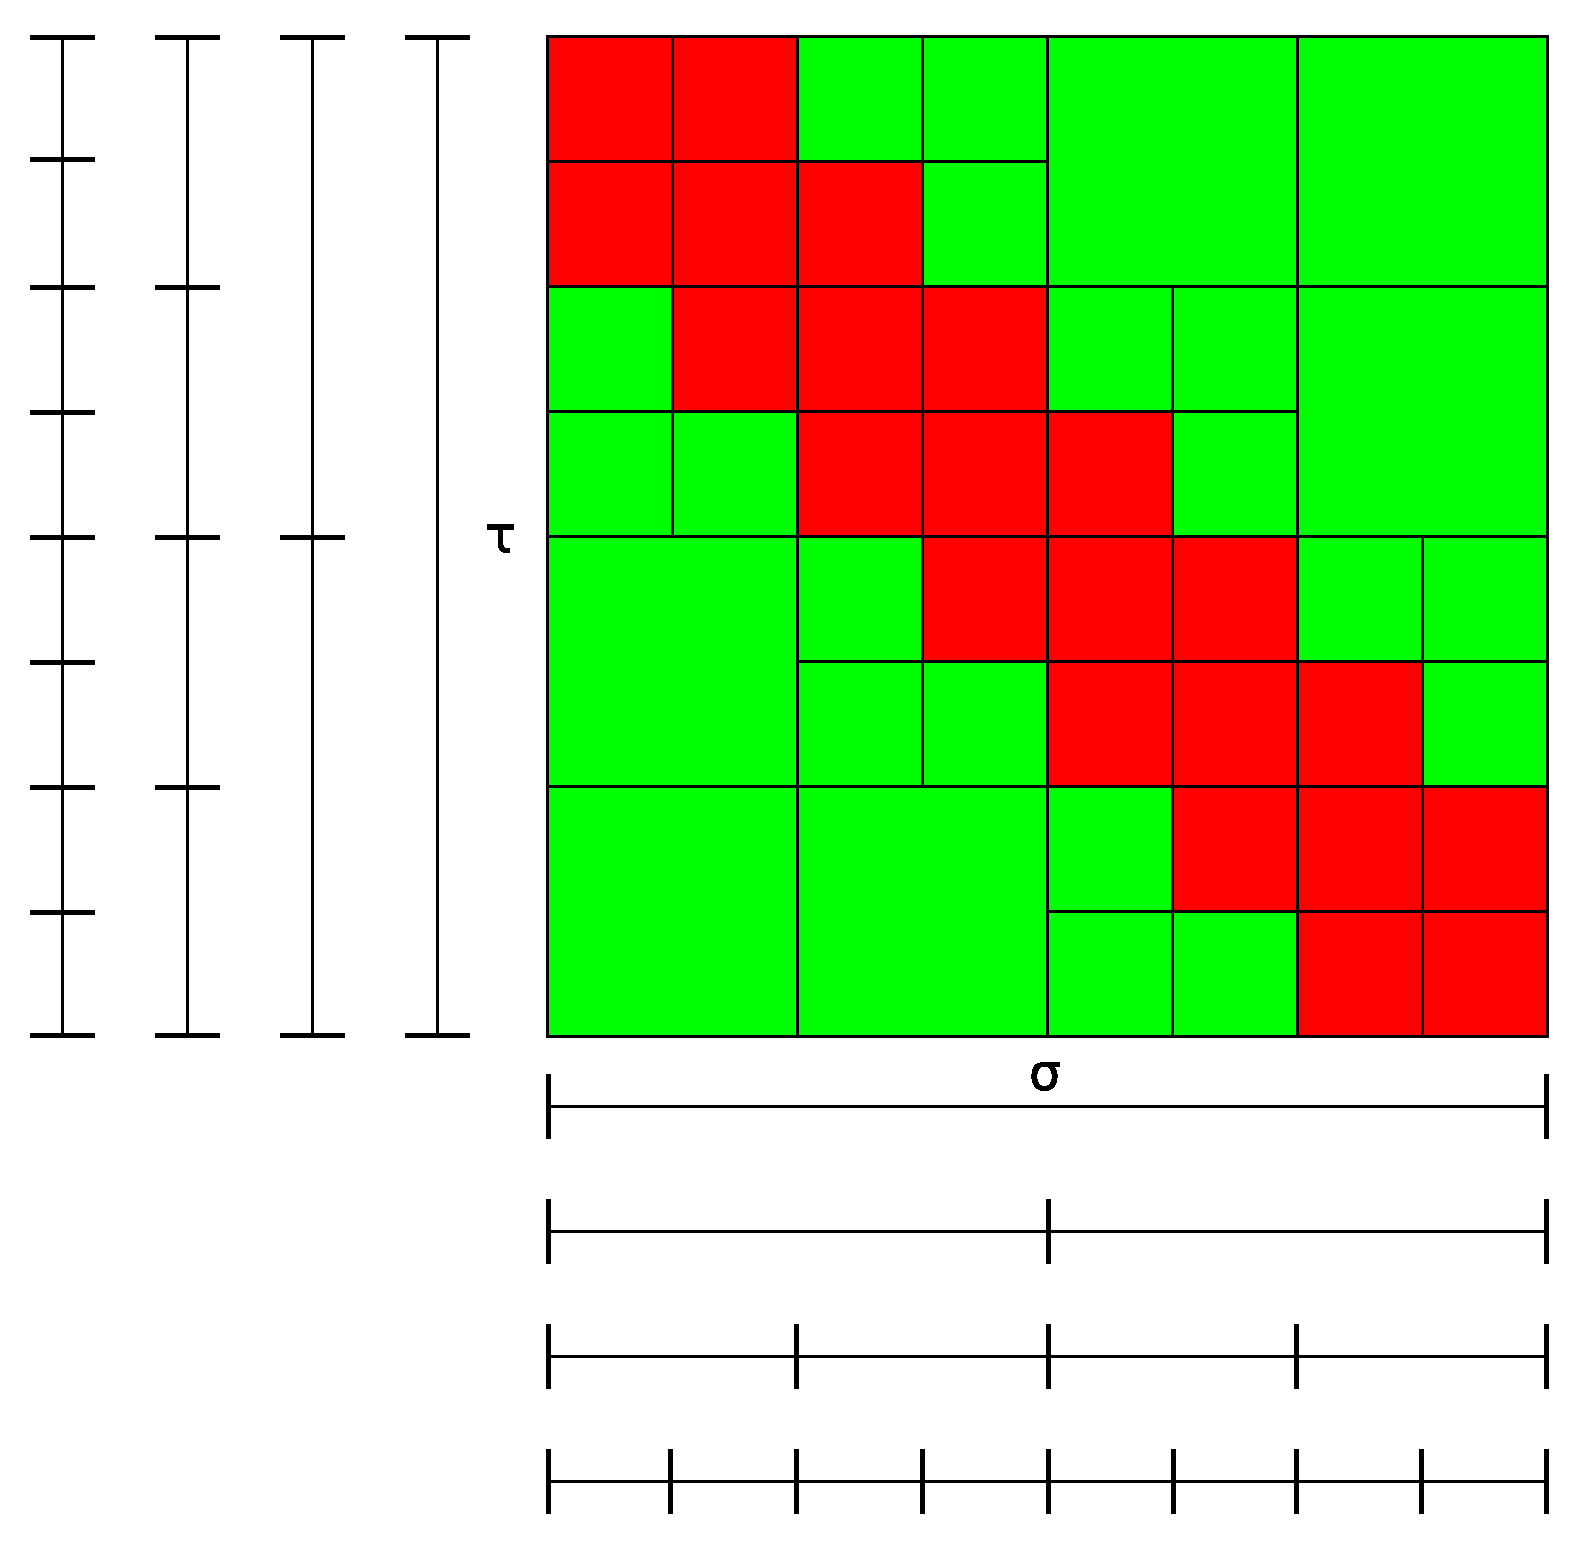
\includegraphics[width=.5\linewidth]{figures/fg-h2-matrix.pdf}\caption{Aufbau eineer \(\mathcal{H}^2\)-Matrix aus Clusterbasen \(\tau\) und \(\sigma\)}
      \onslide<2>\centering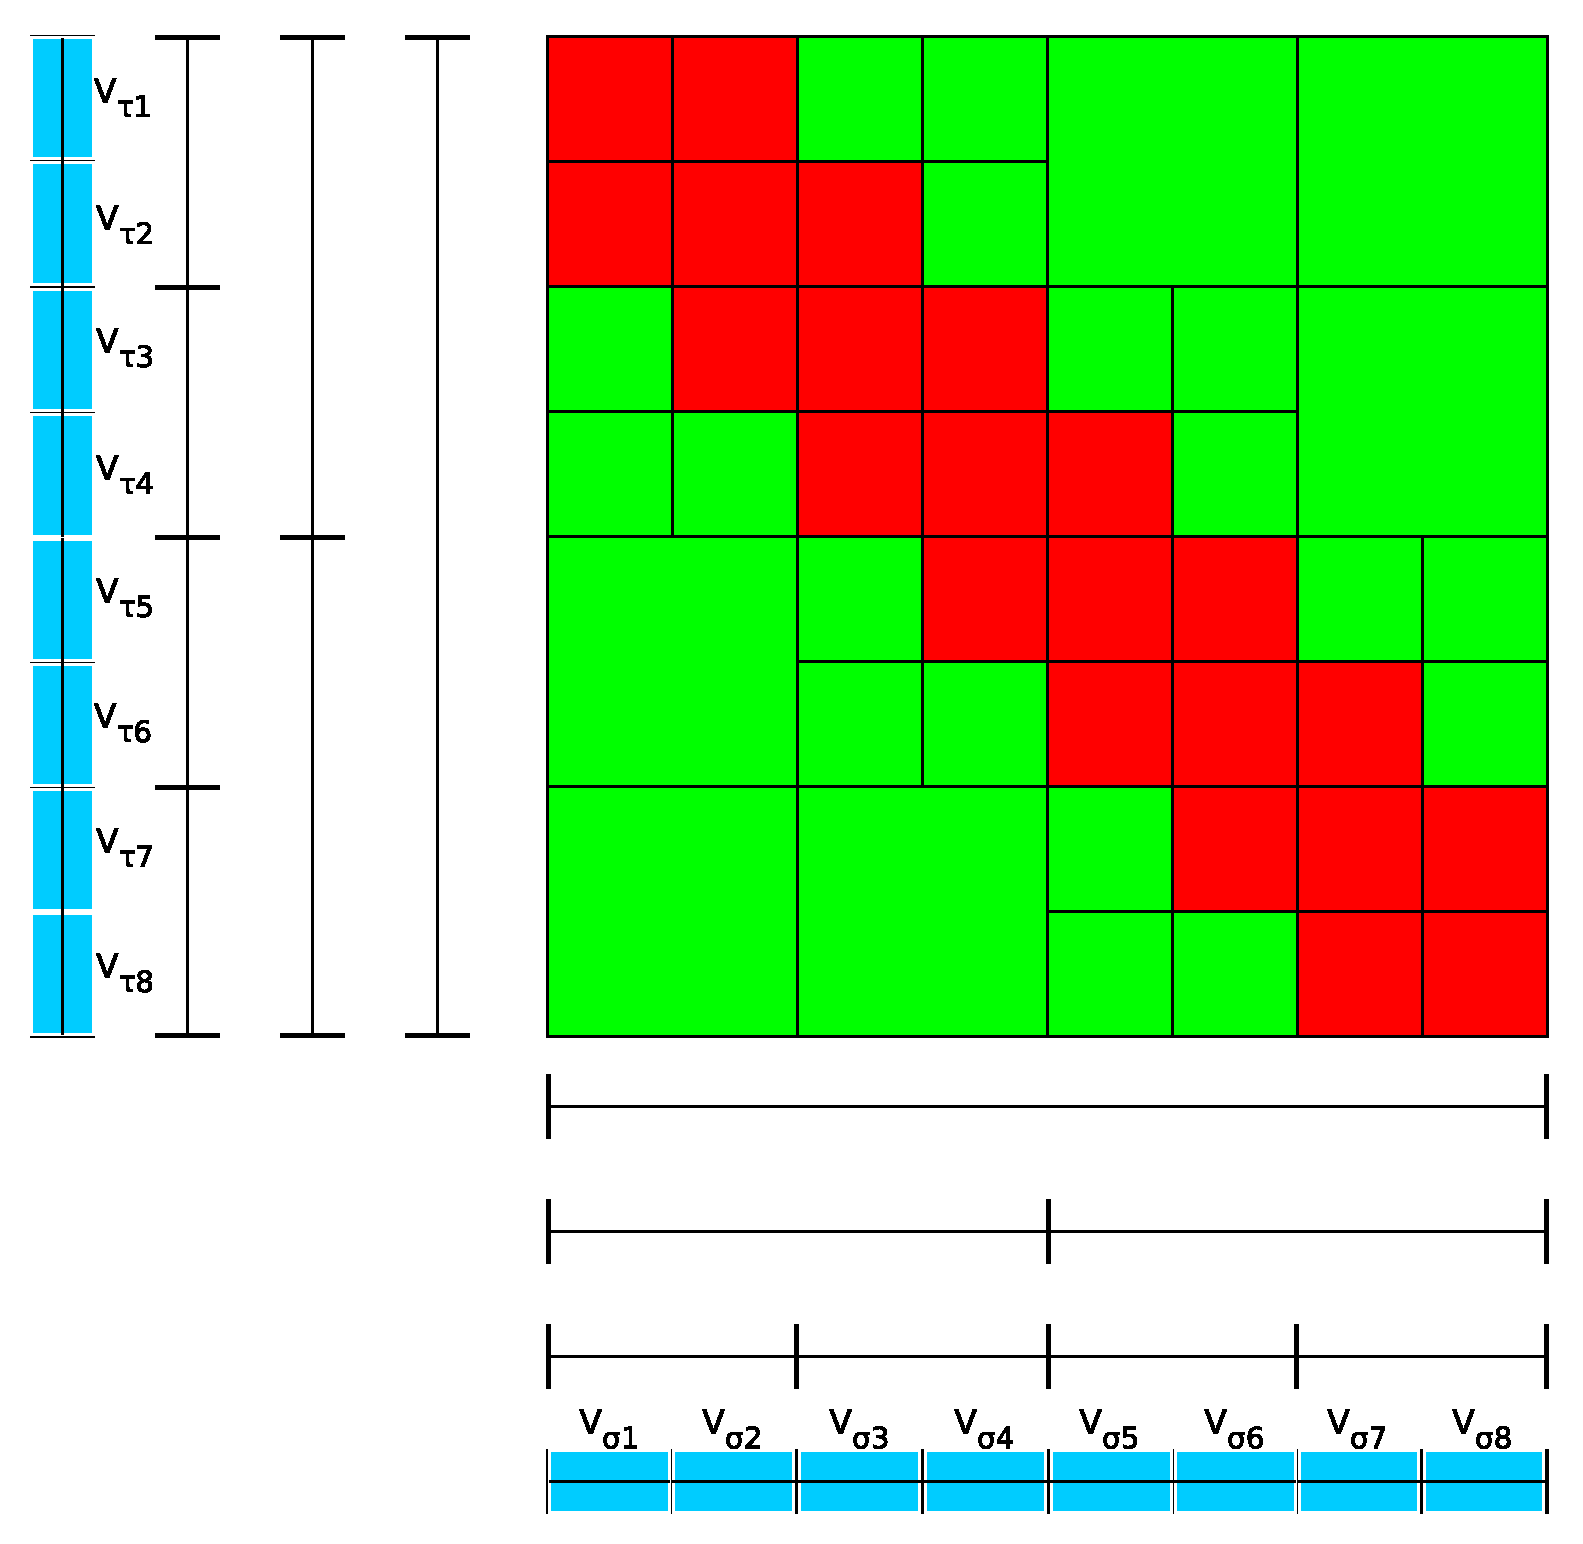
\includegraphics[width=.5\linewidth]{figures/fg-h2-leaf-matrices.pdf}\caption{Blattmatrizen der Clusterbasen \(\tau\) und \(\sigma\)}
      \onslide<3>\centering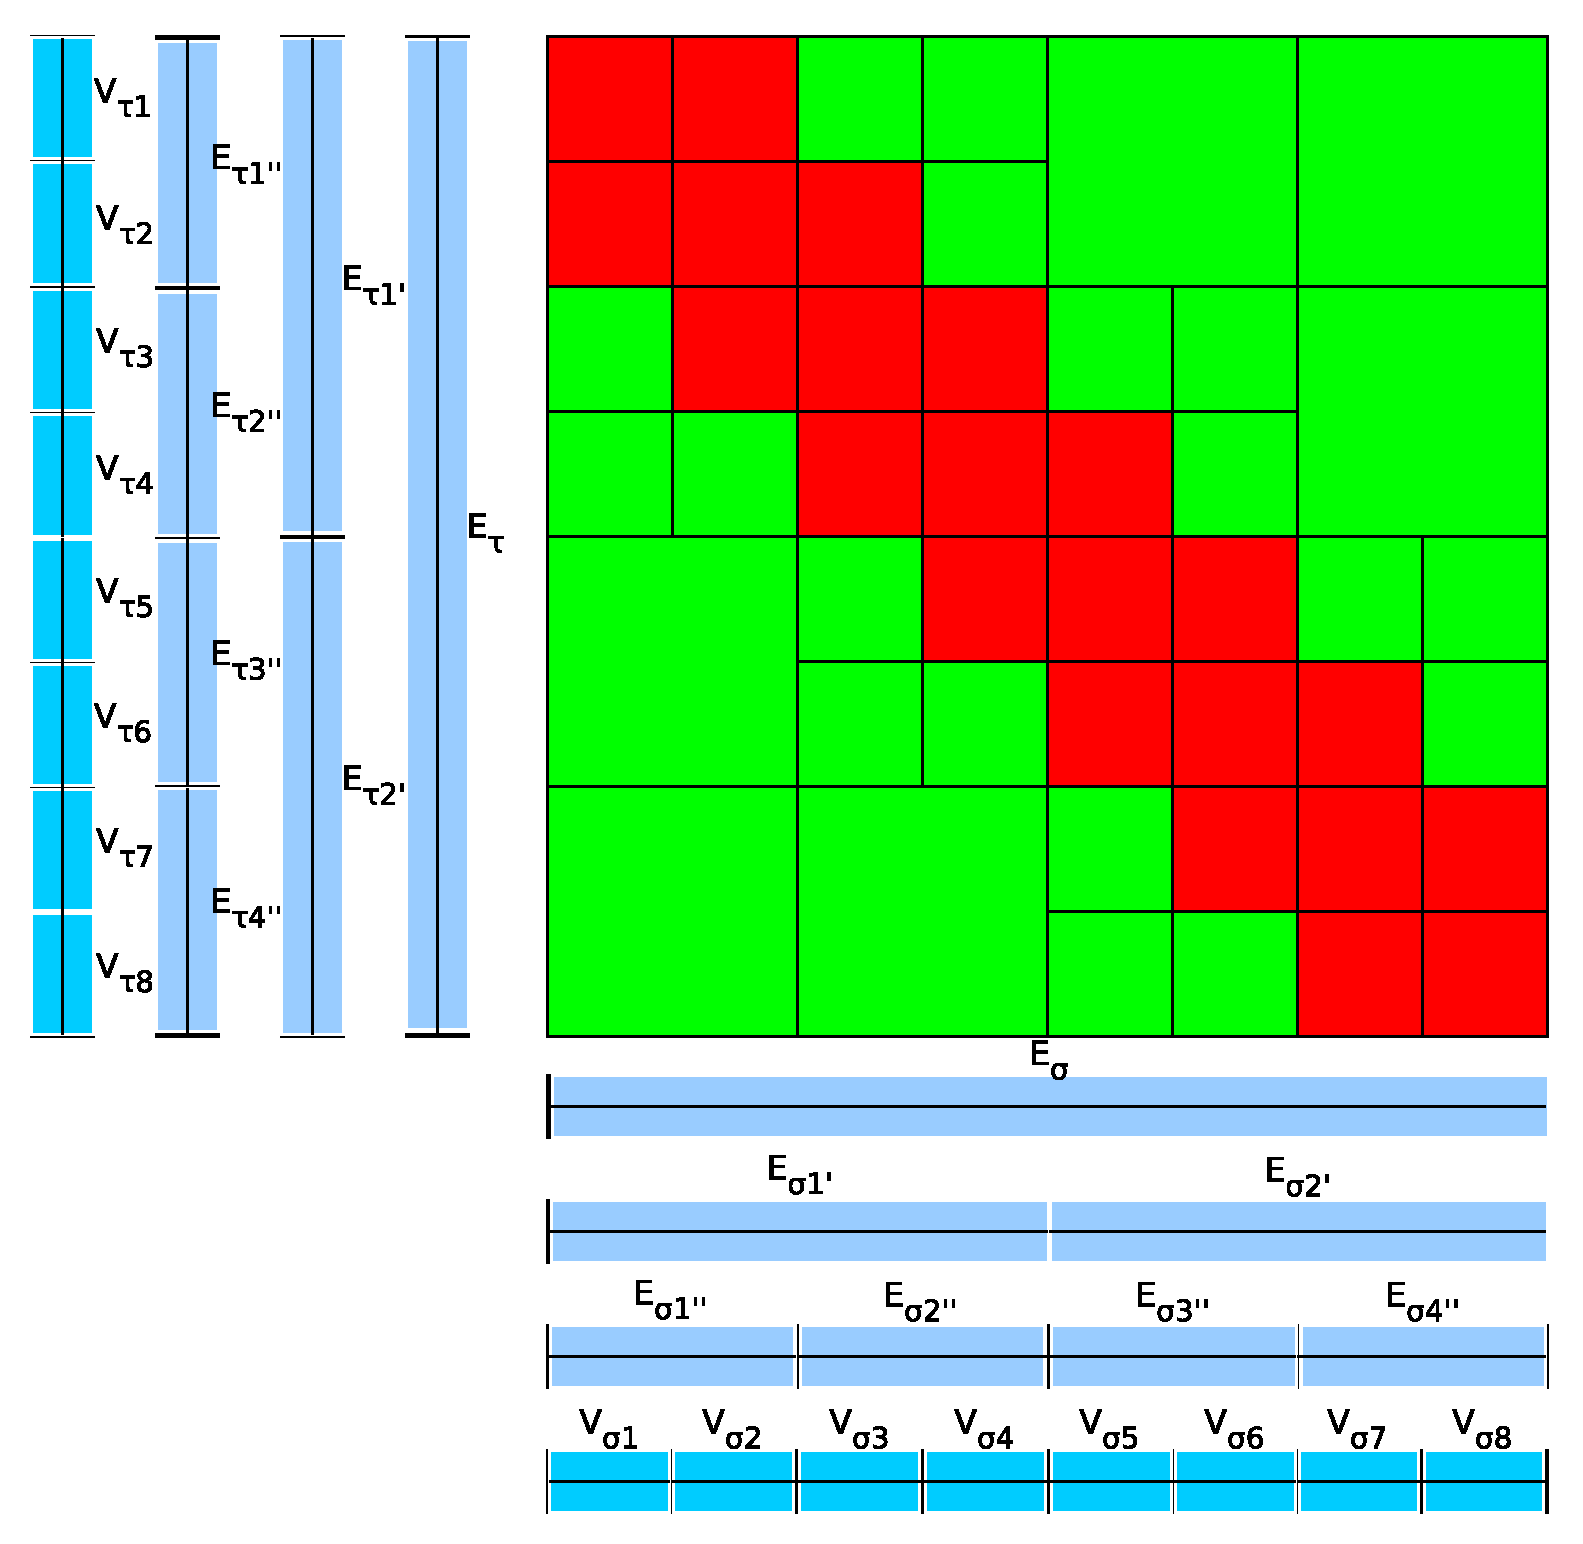
\includegraphics[width=.5\linewidth]{figures/fg-h2-transfer-matrices.pdf}\caption{Aufbau der Teilclusterbasen von \(\tau\) und \(\sigma\)}
      \onslide<4>\centering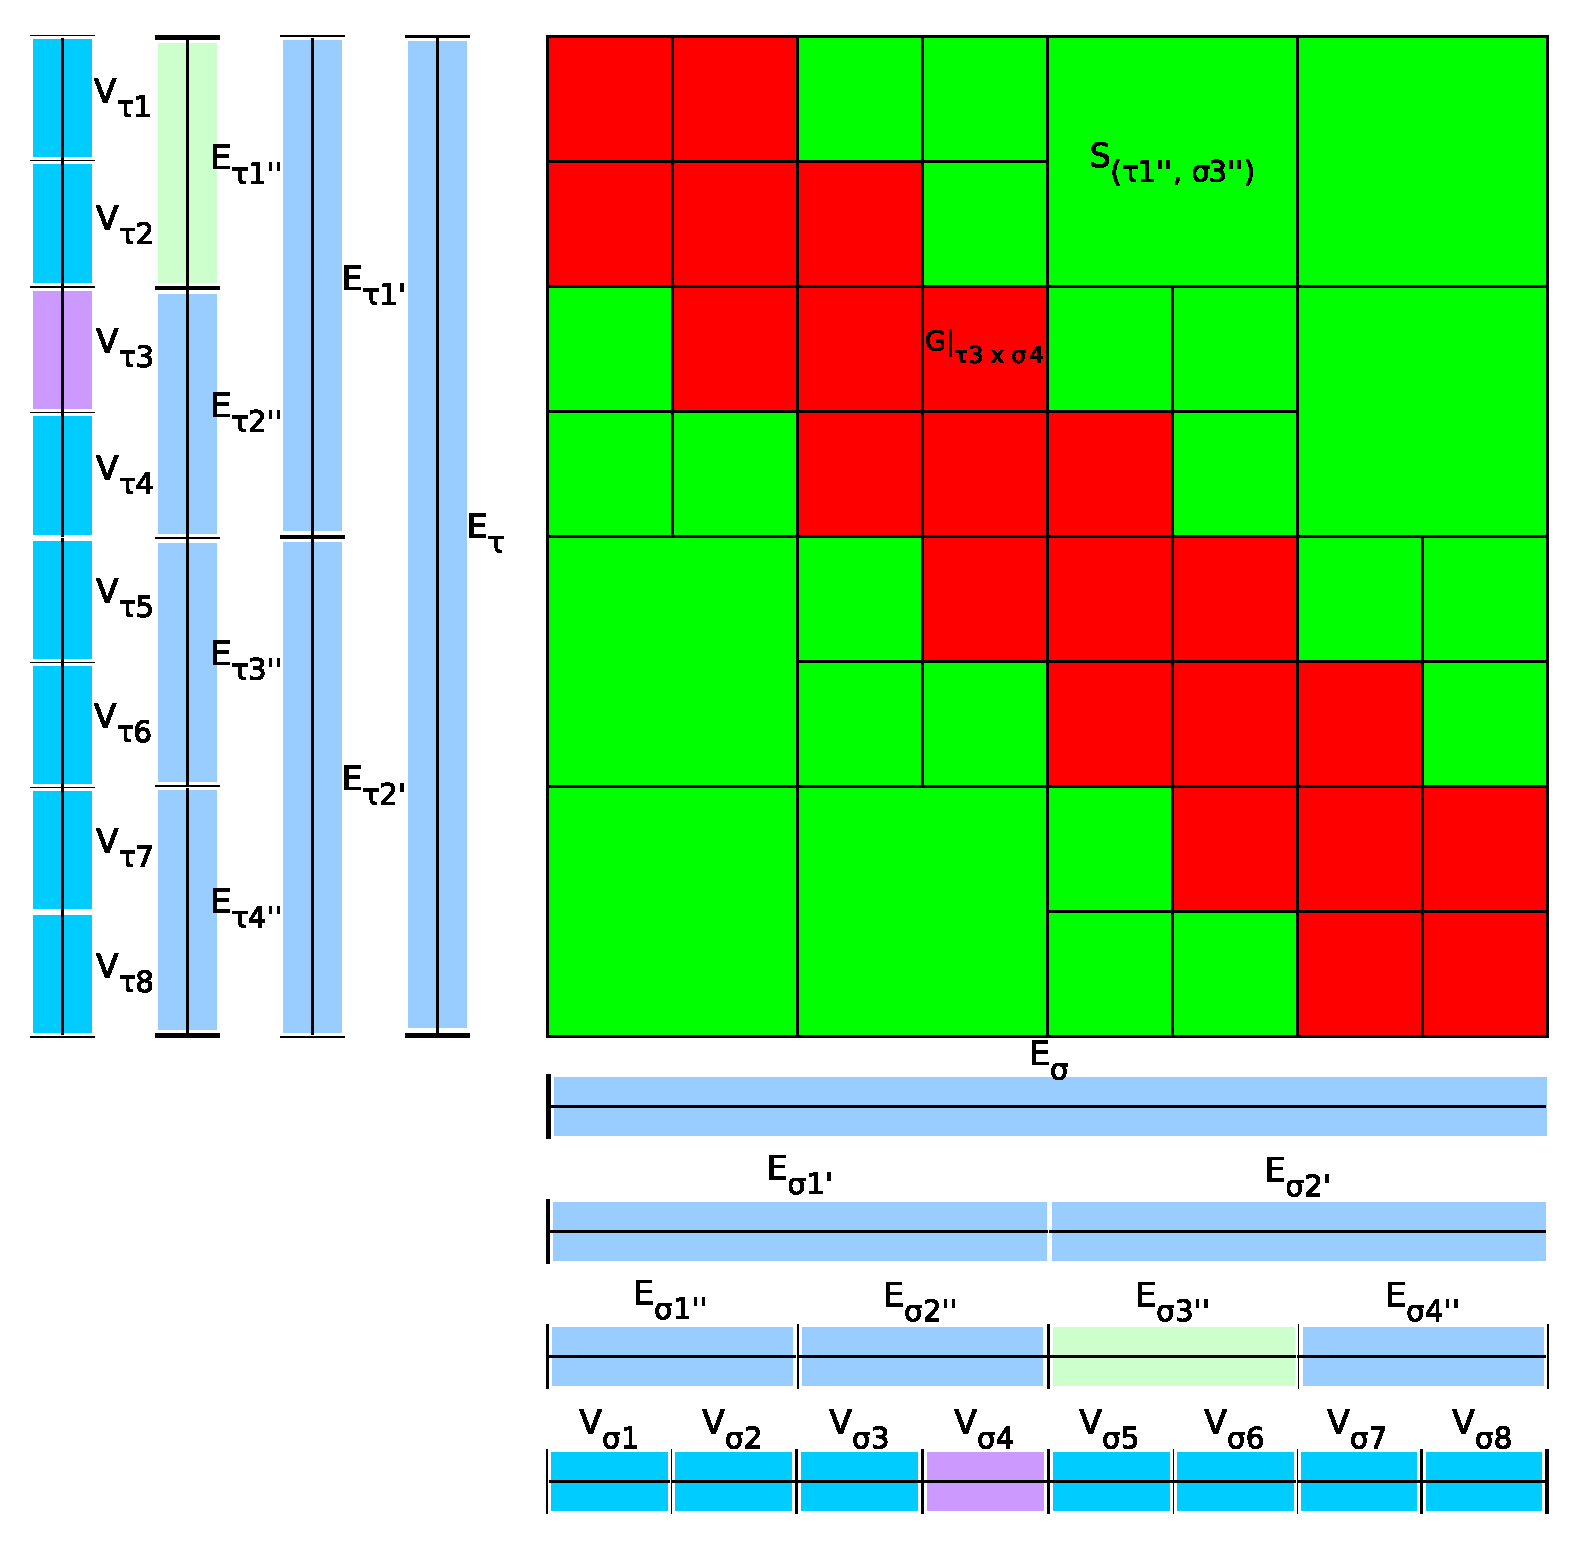
\includegraphics[width=.5\linewidth]{figures/fg-h2-near-far-field-matrices.pdf}\caption{Matrizen für zulässige und unzulässige Blöcke}
    \end{overprint}
  \end{figure}

  \footnotesize
  \let\thefootnote\relax\footnote{Quelle: \href{https://link.springer.com/article/10.1007\%2Fs00607-002-1450-4?LI=true}{Data-sparse approximation by adaptive \(\mathcal{H}^2\)-matrices.}}
  \addtocounter{footnote}{-1}\let\thefootnote\svthefootnote\relax
  \normalsize
\end{frame}

\begin{frame}{\(\mathcal{H}^2\)-Matrizen}
  \begin{itemize}
    \item Sei \(\tilde{G}|_{\hat{\tau} \times \hat{\sigma}} =
    \begin{cases}
      V_{\tau} S_{\tau \sigma} V_{\sigma}^T & \tau \times \sigma \text{ zulässig} \\
      G|_{\hat{\tau} \times \hat{\sigma}}   & sonst
    \end{cases}\)
    \begin{itemize}
      \item Seien \(\hat{\tau}\) und \( \hat{\sigma}\) die Indexmengen von \(\tau\) und \(\sigma\)
    \end{itemize}
    \item \(V_{\tau}\) existiert, falls \(\tau\) ein Blatt ist
    \item Ansonsten gilt \(V_{\tau}|_{\hat{\tau} '} = V_{\tau '} E_{\tau '}\) für alle  \(\tau ' \in sons(\tau)\)
    \item \(V_{\sigma}\) ist analog definiert
  \end{itemize}

  \footnotesize
  \let\thefootnote\relax\footnote{Quelle: \href{https://link.springer.com/article/10.1007\%2Fs00607-002-1450-4?LI=true}{Data-sparse approximation by adaptive \(\mathcal{H}^2\)-matrices.}}
  \addtocounter{footnote}{-1}\let\thefootnote\svthefootnote\relax
  \normalsize
\end{frame}

\begin{frame}{\(\mathcal{H}^2\)-Matrix-Vektor-Multiplikation}
  \begin{columns}
    \column{.33\linewidth}
      \begin{overprint}
        \onslide<1>
          \(y|_{\hat{\tau}} := \overbrace{V_{\tau} \underbrace{S_{\tau \sigma}
            \overbrace{V_{\sigma}^T
            x|_{\hat{\sigma}}}^{\textcolor{red}{\text{forward}}}}_{fastaddeval}}
            ^{backward}\)
        \onslide<2>
          \(y|_{\hat{\tau}} := \overbrace{V_{\tau} \underbrace{S_{\tau \sigma}
            \textcolor{orange}{\hat{x}_\sigma}}_{\textcolor{red}{fastaddeval}}}
            ^{backward}\)
        \onslide<3>
          \(y|_{\hat{\tau}} := \overbrace{V_{\tau}
            \textcolor{orange}{\hat{y}_\tau}}^{\textcolor{red}{backward}}\)
      \end{overprint}

    \column{.5\linewidth}
      \begin{overprint}
        \onslide<1>
          \begin{algorithm}[H]
            \begin{algorithmic}[1]
              \normalsize
              {
              \Function{Forward}{cluster \(\sigma\)}
              \If{\(sons(\sigma) = \emptyset\)}
                \State{\(\hat{x}_{\sigma} \leftarrow V^T_{\sigma} x|_{\hat{\sigma}}\)}
              \Else{}
                \State{\(\hat{x}_{\sigma} \leftarrow 0\)}
                \For{\(\sigma' \in sons(\sigma)\)}
                  \State{FORWARD\relax(\(\sigma'\))}
                  \State{\(\hat{x}_{\sigma} \leftarrow \hat{x}_{\sigma} +
                           E^T_{\sigma'}\hat{x}_{\sigma'}\)}
                \EndFor{}
              \EndIf{}
              \EndFunction{}
              }
            \end{algorithmic}
          \end{algorithm}
      \onslide<2>
        \begin{algorithm}[H]
          \begin{algorithmic}[1]
            \normalsize
            {
            \Function{fastaddeval}{}
            \State{(\(\alpha\), block \(, b = (\tau, \sigma)\))}
            \If{\(b \in \mathcal{L}_{\mathcal{I} \times \mathcal{J}}^{+}\)}
              \State{\(\hat{y}_{\tau} \leftarrow \hat{y}_{\tau} + \alpha S_{b}
                       \hat{x}_{\sigma}\)}
            \ElsIf{\(b \in \mathcal{L}_{\mathcal{I} \times \mathcal{J}}^{-}\)}
              \State{\(y|_{\hat{\tau}} \leftarrow y|_{\hat{\tau}} + \alpha
                       G|_{\hat{\tau} \times \hat{\sigma}} x|_{\hat{\sigma}}\)}
            \Else{}
              \For{\(b' \in sons(b)\)}
                \State{FASTADDEVAL\relax(\(\alpha, b'\))}
              \EndFor{}
            \EndIf{}
          \EndFunction{}
          }
          \end{algorithmic}
        \end{algorithm}
      \onslide<3>
      \begin{algorithm}[H]
        \begin{algorithmic}[1]
          \normalsize
          {
          \Function{Backward}{cluster \(\tau\)}
          \If{\(sons(\tau) = \emptyset\)}
            \State{\(y|_{\hat{\tau}} \leftarrow y|_{\hat{\tau}} + V_{\tau}
                     \hat{y}_{\tau}\)}
          \Else{}
            \For{\(\tau' \in sons(\tau)\)}
              \State{\(\hat{y}_{\tau'} \leftarrow \hat{y}_{\tau'} +
                       E_{\tau'}\hat{y}_{\tau}\)}
              \State{Backward\relax(\(\tau'\))}
            \EndFor{}
          \EndIf{}
          \EndFunction{}
          }
        \end{algorithmic}
      \end{algorithm}
    \end{overprint}
  \end{columns}

  \footnotesize
  \let\thefootnote\relax\footnote{Quelle: \href{https://link.springer.com/article/10.1007\%2Fs00607-002-1450-4?LI=true}{Data-sparse approximation by adaptive \(\mathcal{H}^2\)-matrices.}}
  \addtocounter{footnote}{-1}\let\thefootnote\svthefootnote\relax
  \normalsize
\end{frame}

\section{GCA-Methode}

\begin{frame}{GCA-Methode}
  \begin{enumerate}
    \item Niedrigrangapproximation eines zulässigen Blocks durch Greens zweite
          Identität
  \end{enumerate}

  \begin{overprint}
      \onslide<1>
        \begin{itemize}
          \item \(g(x, y) = \int\limits_{\partial \omega} g(x, z)
                  \frac{\partial g}{\partial n(z)}(z, y) \ dz \ -
                  \int\limits_{\partial \omega}
                  \frac{\partial g}{\partial n(z)}(x, z) g(z, y) \ dz\)
          \item[] \hfil für alle \(x \in \omega, y \notin \omega\)
        % \item \visible<2->{\(G|_{\hat{\tau} \times \hat{\sigma}} \approx
        %                      A_{\tau} B_{\tau\omega}^{*} \qquad A_{\tau} =
        %                      (A_{\tau+} A_{\tau-}) \qquad B_{\tau\sigma} =
        %                      (B_{\tau\sigma+} B_{\tau\sigma-})\)}
        \end{itemize}
      \onslide<2>
        \begin{itemize}
          \item \(G|_{\hat{\tau} \times \hat{\sigma}} \approx A_{\tau}
                  B_{\tau\omega}^{*} \qquad A_{\tau} = (A_{\tau+} \ A_{\tau-})
                  \qquad B_{\tau\sigma} = (B_{\tau\sigma+} \ B_{\tau\sigma-})\)
          \item[] \hfil \(A_{\tau+}, A_{\tau-} \in \mathbb{R}^{\hat{\tau}
                  \times K}, B_{\tau\sigma+}, B_{\tau\sigma-} \in
                  \mathbb{R}^{\hat{\sigma} \times K}\)
          \item[] \hfil \(K := \{1, \hdots, 2d \} \times \{1, \hdots, m\}^{d-1},
                  m \in \mathbb{N}\)
          \begin{align*}
            a_{\tau+, i, \nu} &:= w_{\nu} \int\limits_{\Omega} \varphi_{i}(x)
                                  g(x, z_{\nu}) dx, && b_{\tau\sigma+, j\nu} &:=
                                  \int\limits_{\Omega} \psi_{j}(y)
                                  \frac{\partial g}{\partial n_{\iota}}
                                  (z_{\nu}, y) \ dy \\
            a_{\tau-, i, \nu} &:= w_{\nu} \int\limits_{\Omega} \varphi_{i}(x)
                                  \frac{\partial g}{\partial n_{\iota}}
                                  (x, z_{\nu}) dx, && b_{\tau\sigma-, j\nu} &:=
                                  -\int\limits_{\Omega} \psi_{j}(y)
                                  g(z_{\nu}, y) \ dy
          \end{align*}
          \item[] \hfil \(\nu = (\iota, \mu) \in K, i \in \hat{\tau}, j \in
                          \hat{\sigma}, w_{\nu} \in \mathbb{R}, z \in
                          \mathbb{R}^{d}\)
        \end{itemize}
  \end{overprint}

  \footnotesize
  \let\thefootnote\relax\footnote{Quelle: \href{https://link.springer.com/article/10.1007\%2Fs00211-015-0757-y}{Approximation of integral operators by Green quadrature and nested cross approximation}}
  \addtocounter{footnote}{-1}\let\thefootnote\svthefootnote\relax
  \normalsize
\end{frame}

\begin{frame}{Kreuzapproximationsmethode}
  \begin{itemize}
    \item \visible<1->{\(i_{1} \in \hat{\tau}, j_{1} \in \hat{\sigma} \qquad
                         c_{i}^{(1)} := \frac{x_{i, j_{1}}}{x_{i_{1}, j_{1}}}
                         \qquad d_{j}^{(1)} := x_{i_{1}, j}\)}
    \item[] \visible<1->{\hfil \(\tilde{X}^{(1)} := c^{(1)} (d^{(1)})^{*}\)}
    \item \visible<2->{Bereche ab, wenn der Fehler (\(X^{(1)} := X -
                       \tilde{X}^{(1)}\)) klein genug ist, ansonsten wiederhole
                       Prozedur mit \(X^{(1)}\).}
    \item \visible<3->{\(X = CD^{*} = (c^{(1)} \hdots c^{(l)}) (d^{(1)} \hdots
                         d^{(l)})^{*}\)}
  \end{itemize}

  \footnotesize
  \let\thefootnote\relax\footnote{Quelle: \href{https://link.springer.com/article/10.1007\%2Fs00211-015-0757-y}{Approximation of integral operators by Green quadrature and nested cross approximation}}
  \addtocounter{footnote}{-1}\let\thefootnote\svthefootnote\relax
  \normalsize
\end{frame}

\begin{frame}{Algebraische Interpolation}
  \begin{itemize}
    \item \visible<1->{Zeilenpermuationsmatrix \(P \in \mathbb{R}^{l \times
                         \hat{\tau}}\)}
    \item[] \visible<1->{\hfil \(Pz :=
                                 \begin{pmatrix}
                                   z_{i_{1}} \\
                                   \vdots \\
                                   z_{i_{l}}
                                 \end{pmatrix}
                                 \qquad \text{für alle } z \in \mathbb{R}^{\tau}
                               \)}
    \item \visible<2->{\(V := C{(PC)}^{-1} \qquad \mathfrak{J} := VP\)}
    \item \visible<3->{\(\mathfrak{I}C = VPC = C{(PC)}^{-1}PC = C\)}
    \item \visible<3->{\(\mathfrak{I}X = VPX = VPCD^{*} = CD^{*}\)}
  \end{itemize}

  \footnotesize
  \let\thefootnote\relax\footnote{Quelle: \href{https://link.springer.com/article/10.1007\%2Fs00211-015-0757-y}{Approximation of integral operators by Green quadrature and nested cross approximation}}
  \addtocounter{footnote}{-1}\let\thefootnote\svthefootnote\relax
  \normalsize
\end{frame}

\begin{frame}{GCA-Methode}
  \begin{enumerate}
    \item \visible<1->{Niedrigrangapproximation eines zulässigen Blocks durch
                       Greens zweite Identität}
    \item \visible<1->{Approximation von \(A_{\tau}\) mithilfe der
                       Kreuzapproximationsmethode}
    \item \visible<2->{Wiederhole 1.\ und 2.\ für
                       \(G|_{\hat{\tau} \times \hat{\sigma}}^{*}\) }
    \item \visible<3->{Wende Kreuzapproximation auf permutierte Nicht-Blätter
                       an}
  \end{enumerate}

  \begin{overprint}
      \onslide<1>
        \begin{itemize}
          \item \(A_{t} \approx C_{\tau}D_{\tau}^{*} = \mathfrak{I}A_{\tau} =
                  V_{\tau}P_{\tau}A_{\tau} \qquad G|_{\hat{\tau} \times \hat{\sigma}} \approx V_{\tau}P_{\tau}
                  G|_{\hat{\tau} \times \hat{\sigma}}\)
        \end{itemize}
      \onslide<2>
        \begin{itemize}
          \item \(G|_{\hat{\tau} \times \hat{\sigma}} \approx V_{\tau}
                  \underbrace{P_{\tau}G|_{\hat{\tau} \times \hat{\sigma}}P_{\sigma}^{*}}_{S_{b}}
                  V_{\sigma}^{*}\)
        \end{itemize}
      \onslide<3>
        \begin{itemize}
          \small
          \item \(\begin{pmatrix}
                    V_{\tau 1} & \\
                               & V_{\tau 2}
                  \end{pmatrix}
                  \begin{pmatrix}
                    P_{\tau 1} & \\
                               & P_{\tau 2}
                  \end{pmatrix} A_{\tau} \approx
                  \begin{pmatrix}
                    V_{\tau 1} & \\
                               & V_{\tau 2}
                  \end{pmatrix} \widehat{V}_{\tau}\widehat{P}_{\tau}
                  \begin{pmatrix}
                    P_{\tau 1} & \\
                               & P_{\tau 2}
                  \end{pmatrix} A_{\tau}\)
          \normalsize
          \item \( \begin{pmatrix}
                     E_{\tau 1} \\ E_{\tau 2}
                   \end{pmatrix} := \widehat{V}_{\tau} \Rightarrow V_{\tau} :=
                   \begin{pmatrix}
                      V_{\tau 1} & \\
                                 & V_{\tau 2}
                   \end{pmatrix}\widehat{V}_{\tau} =
                   \begin{pmatrix}
                     V_{\tau 1} E_{\tau 1} \\ V_{\tau 2} E_{\tau 2}
                   \end{pmatrix}\)
        \end{itemize}
  \end{overprint}

  \footnotesize
  \let\thefootnote\relax\footnote{Quelle: \href{https://link.springer.com/article/10.1007\%2Fs00211-015-0757-y}{Approximation of integral operators by Green quadrature and nested cross approximation}}
  \addtocounter{footnote}{-1}\let\thefootnote\svthefootnote\relax
  \normalsize
\end{frame}

\section{GPUs}

\begin{frame}{GPUs}
  \begin{columns}
    \column{0.45\linewidth}
      \begin{itemize}
        \item Graphics Processing Unit (GPU) ist ein auf Bildverarbeitung
              spezialisierter Prozessor
        \begin{itemize}
          \item Schnelle Gleitkommaoperationen
          \item Vektorisierte Architektur
        \end{itemize}
        \item Entwicklung von GPUs durch Videospielindustrie stark
              vorangetrieben
        \item Sehr günstig dank Massenproduktion
      \end{itemize}
    \column{0.45\linewidth}
      \begin{figure}
        \centering
        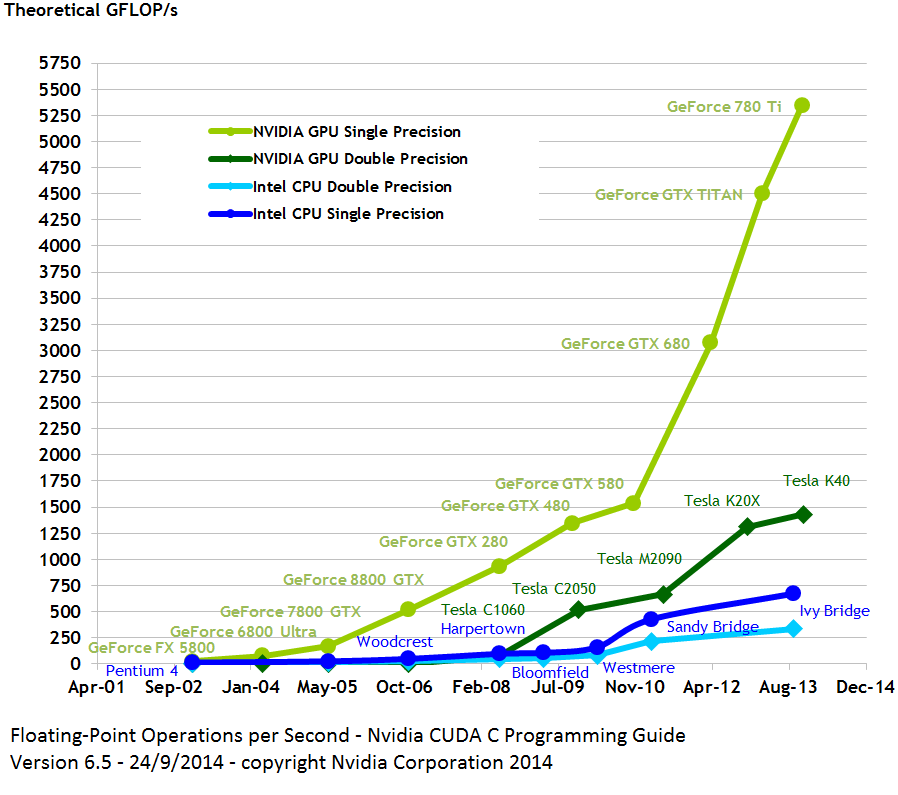
\includegraphics[width=\linewidth]{figures/fg-flops.png}
        \caption{Theoretische Verarbeitungsgeschwindigkeit von
                 Gleitkommaoperationen verschiedener
                 Architekturen\footnotemark[1]}
      \end{figure}
  \end{columns}

  \footnotetext[1]{\url{https://scs.senecac.on.ca/~gpu610/pages/images/flops.png}}
\end{frame}

\begin{frame}{GPUs}
  \begin{figure}
    \centering
    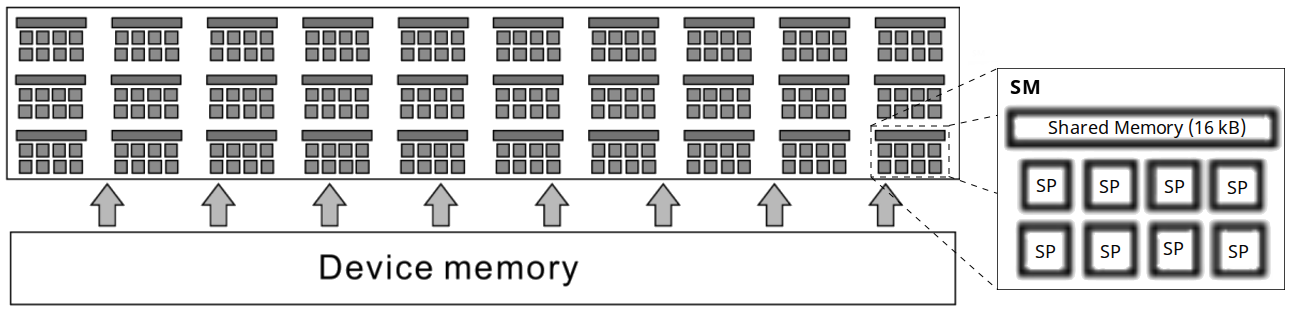
\includegraphics[width=\linewidth]{figures/fg-gpu_architecture.png}
    \caption{Architektur einer Graphikkarte}
  \end{figure}
\end{frame}

\section{OpenCL}

\begin{frame}{OpenCL}
  \begin{itemize}
    \item Framework zum programmieren von/auf unterschiedlichen
          Hardwarearchitekturen
    \begin{itemize}
      \item Field Programmable Gate Arrays (FPGAs)
      \item Digitaler Signalprozessoren (DSPs)
      \item CPUs
      \item GPUs
    \end{itemize}
  \end{itemize}

  \footnotesize
  \let\thefootnote\relax\footnote{Quelle: \href{https://www.khronos.org/registry/OpenCL/specs/opencl-2.0.pdf}{The OpenCL Specifictaion (Version: 2.0)}}
  \addtocounter{footnote}{-1}\let\thefootnote\svthefootnote\relax
  \normalsize
\end{frame}

\begin{frame}{OpenCL}
  \begin{figure}
    \centering
    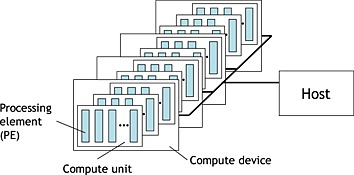
\includegraphics[width=\linewidth]{figures/fg-opencl-platform-model.png}
    \caption{Das Platformmodell von OpenCL\footnotemark[1]}
  \end{figure}

  \footnotesize
  \footnotetext[1]{\url{https://www.researchgate.net/profile/Yi_Ping_You/publication/261411530/figure/fig6/AS:281659619463173@1444164294142/Figure-1-OpenCL-platform-model-adapted-from8.png}}
  \normalsize
\end{frame}

\begin{frame}{OpenCL}
  \begin{figure}
    \centering
    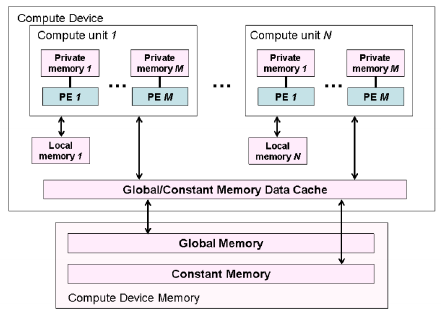
\includegraphics[width=.75\linewidth]{figures/fg-opencl-memory-model.png}
    \caption{Das Speichermodell von OpenCL\footnotemark[1]}
  \end{figure}

  \footnotesize
  \footnotetext[1]{\url{https://www.researchgate.net/publication/275973210_Intelligent_Vehicle_Perception_Toward_the_Integration_on_Embedded_Many-core/figures?lo=1}}
  \normalsize
\end{frame}

\begin{frame}{OpenCL}
  \begin{figure}
    \centering
    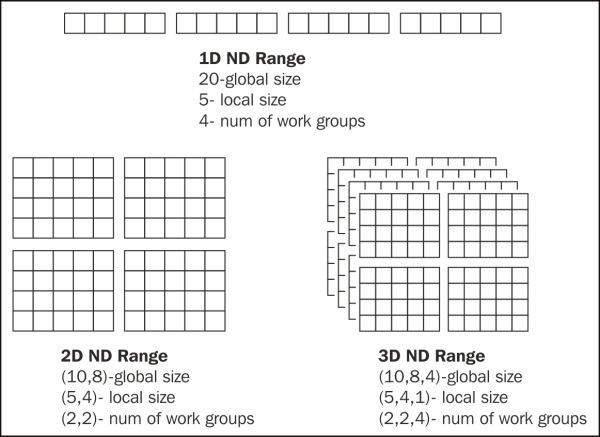
\includegraphics[width=.75\linewidth]{figures/fg-opencl-execution-model.jpg}
    \caption{Das Ausführungsmodell von OpenCL\footnotemark[1]}
  \end{figure}

  \footnotesize
  \footnotetext[1]{\url{https://www.packtpub.com/graphics/9781849692342/graphics/2342OT_02_11.jpg}}
  \normalsize
\end{frame}

\begin{frame}[fragile]{OpenCL}
  \begin{lstlisting}[style=CStyle]
    kernel void vec_inc(global float *a, const float b)
    {
      const size_t gid = get_global_id(0);
      const size_t lid = get_local_id(0);

      local float a_local[32];

      if(lid < 32)
      {
        a_local[lid] = a[gid];

        a_local[lid] += b;

        a[gid] = a_local[lid];
      }
    }
  \end{lstlisting}
\end{frame}
\section{4 Phasen-fastaddeval}

\begin{frame}{Idee}
  \begin{columns}
    \column{.5\linewidth}
      \begin{itemize}
        \item \(S_{b} = P_{\tau}G|_{\tau \times \sigma} P_{\sigma}^{*}\)
        \begin{itemize}
          \item Permutierte Einträge der Galerkin-Diskretisierung
          \item Einträge bestehen nur aus einem Typ von
                Integralen\footnotemark[1]\footnotemark[2]
        \end{itemize}
        \item \(G|_{\hat{\tau} \times \hat{\sigma}}\)
        \begin{itemize}
          \item Einträge der Galerkin-Diskretisierung
          \item Einträge bestehen aus allen Typen von Integralen
        \end{itemize}
      \end{itemize}
    \column{.5\linewidth}
      \begin{algorithm}[H]
        \begin{algorithmic}[1]
          \normalsize
          {
          \Function{fastaddeval}{}
          \State{(\(\alpha\), block \(, b = (\tau, \sigma)\))}
          \If{\(b \in \mathcal{L}_{\mathcal{I} \times \mathcal{J}}^{+}\)}
            \State{\(\hat{y}_{\tau} \leftarrow \hat{y}_{\tau} + \alpha S_{b}
                     \hat{x}_{\sigma}\)}
          \ElsIf{\(b \in \mathcal{L}_{\mathcal{I} \times \mathcal{J}}^{-}\)}
            \State{\(y|_{\hat{\tau}} \leftarrow y|_{\hat{\tau}} + \alpha
                     G|_{\hat{\tau} \times \hat{\sigma}} x|_{\hat{\sigma}}\)}
          \Else{}
            \For{\(b' \in sons(b)\)}
              \State{FASTADDEVAL\relax(\(\alpha, b'\))}
            \EndFor{}
          \EndIf{}
        \EndFunction{}
        }
        \end{algorithmic}
      \end{algorithm}
  \end{columns}
  \footnotesize
  \footnotetext[1]{Typen von Integralen: Keinen gemeinsamen Vertex, einen gemeinsamen Vertex, eine gemeinsame Kante, identisches Dreieck}
  \footnotetext[2]{Quelle: On the efficient computation of singular and nearly singular surface integrals arising in 3D-Galerkin BEM}
  \normalsize
\end{frame}

\begin{frame}{Vorbereitung}\vfill
  \begin{figure}
    \begin{overprint}
      \onslide<1>
        \centering
        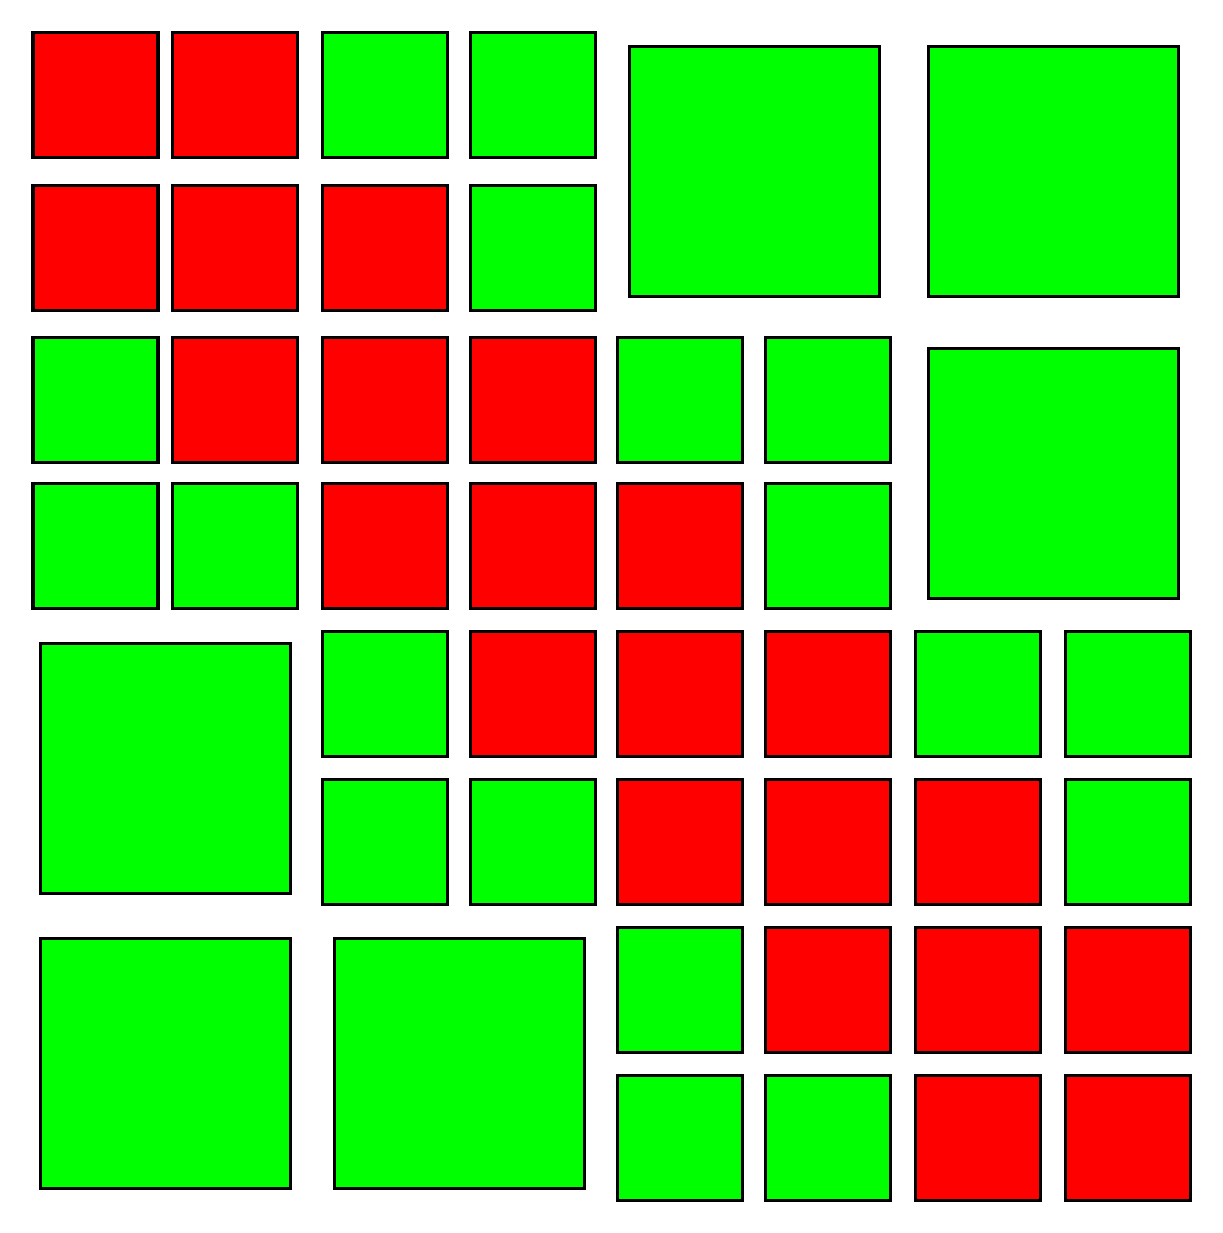
\includegraphics[width=.66\linewidth]{figures/fg-h2-matrix-block.pdf}
        \caption{Betrachte jede Blockmatrix einzeln}
      \onslide<2>
        \centering
        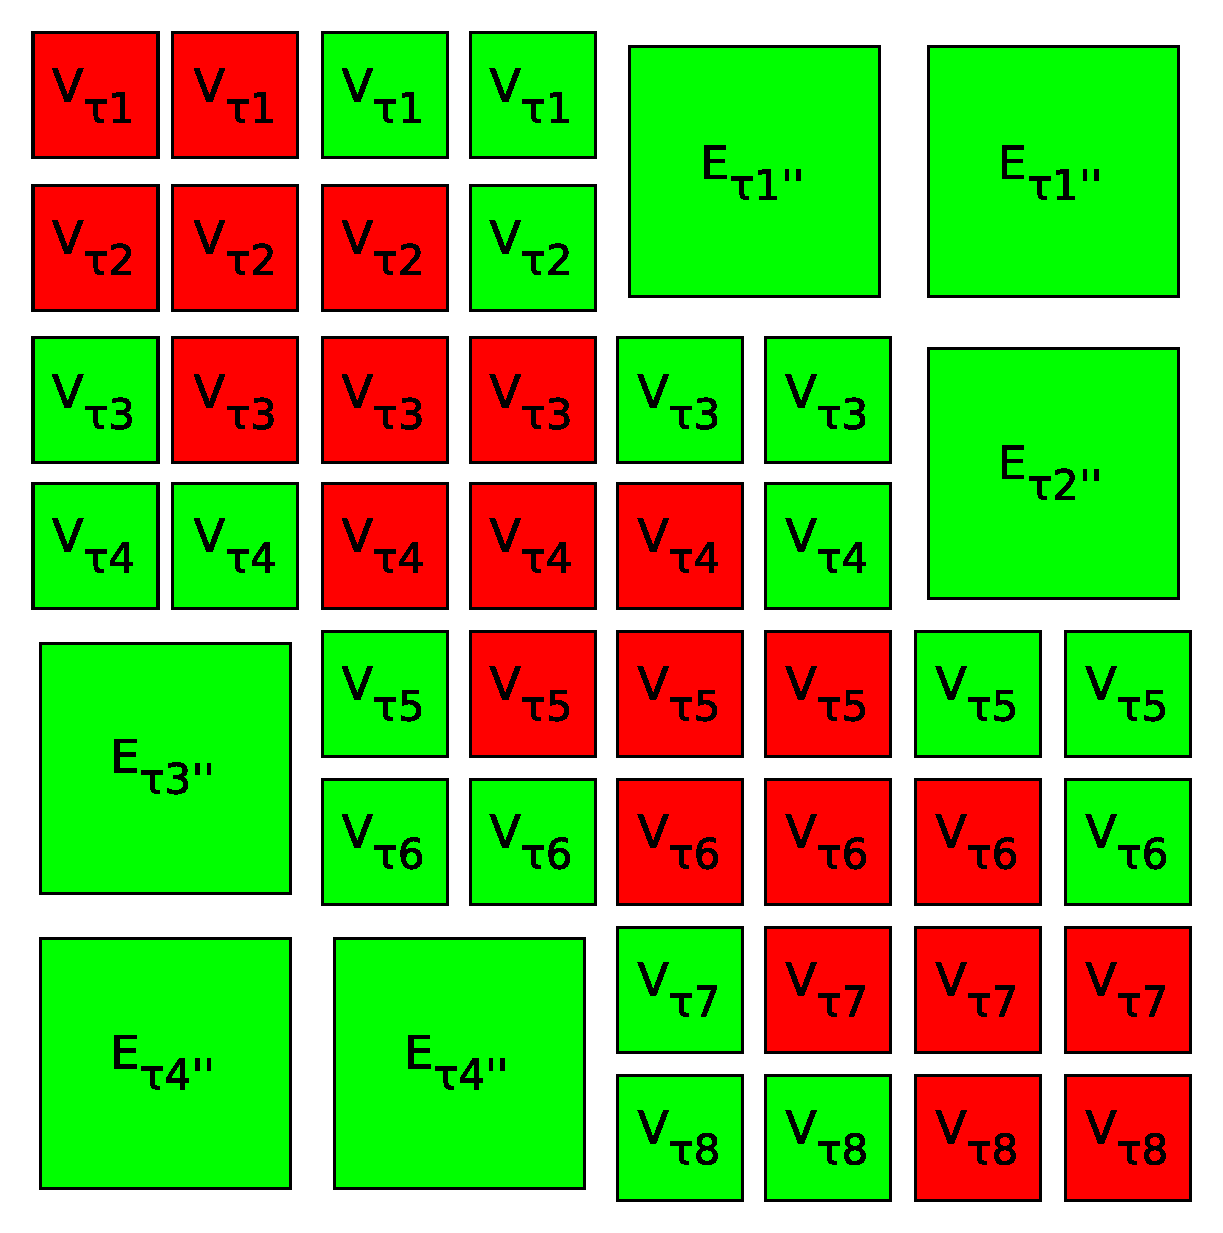
\includegraphics[width=.66\linewidth]{figures/fg-h2-matrix-block-labled.pdf}
        \caption{Kennzeichne die Blockmatrizen mit dem zuständigen Zeilencluster}
      \onslide<3>
        \centering
        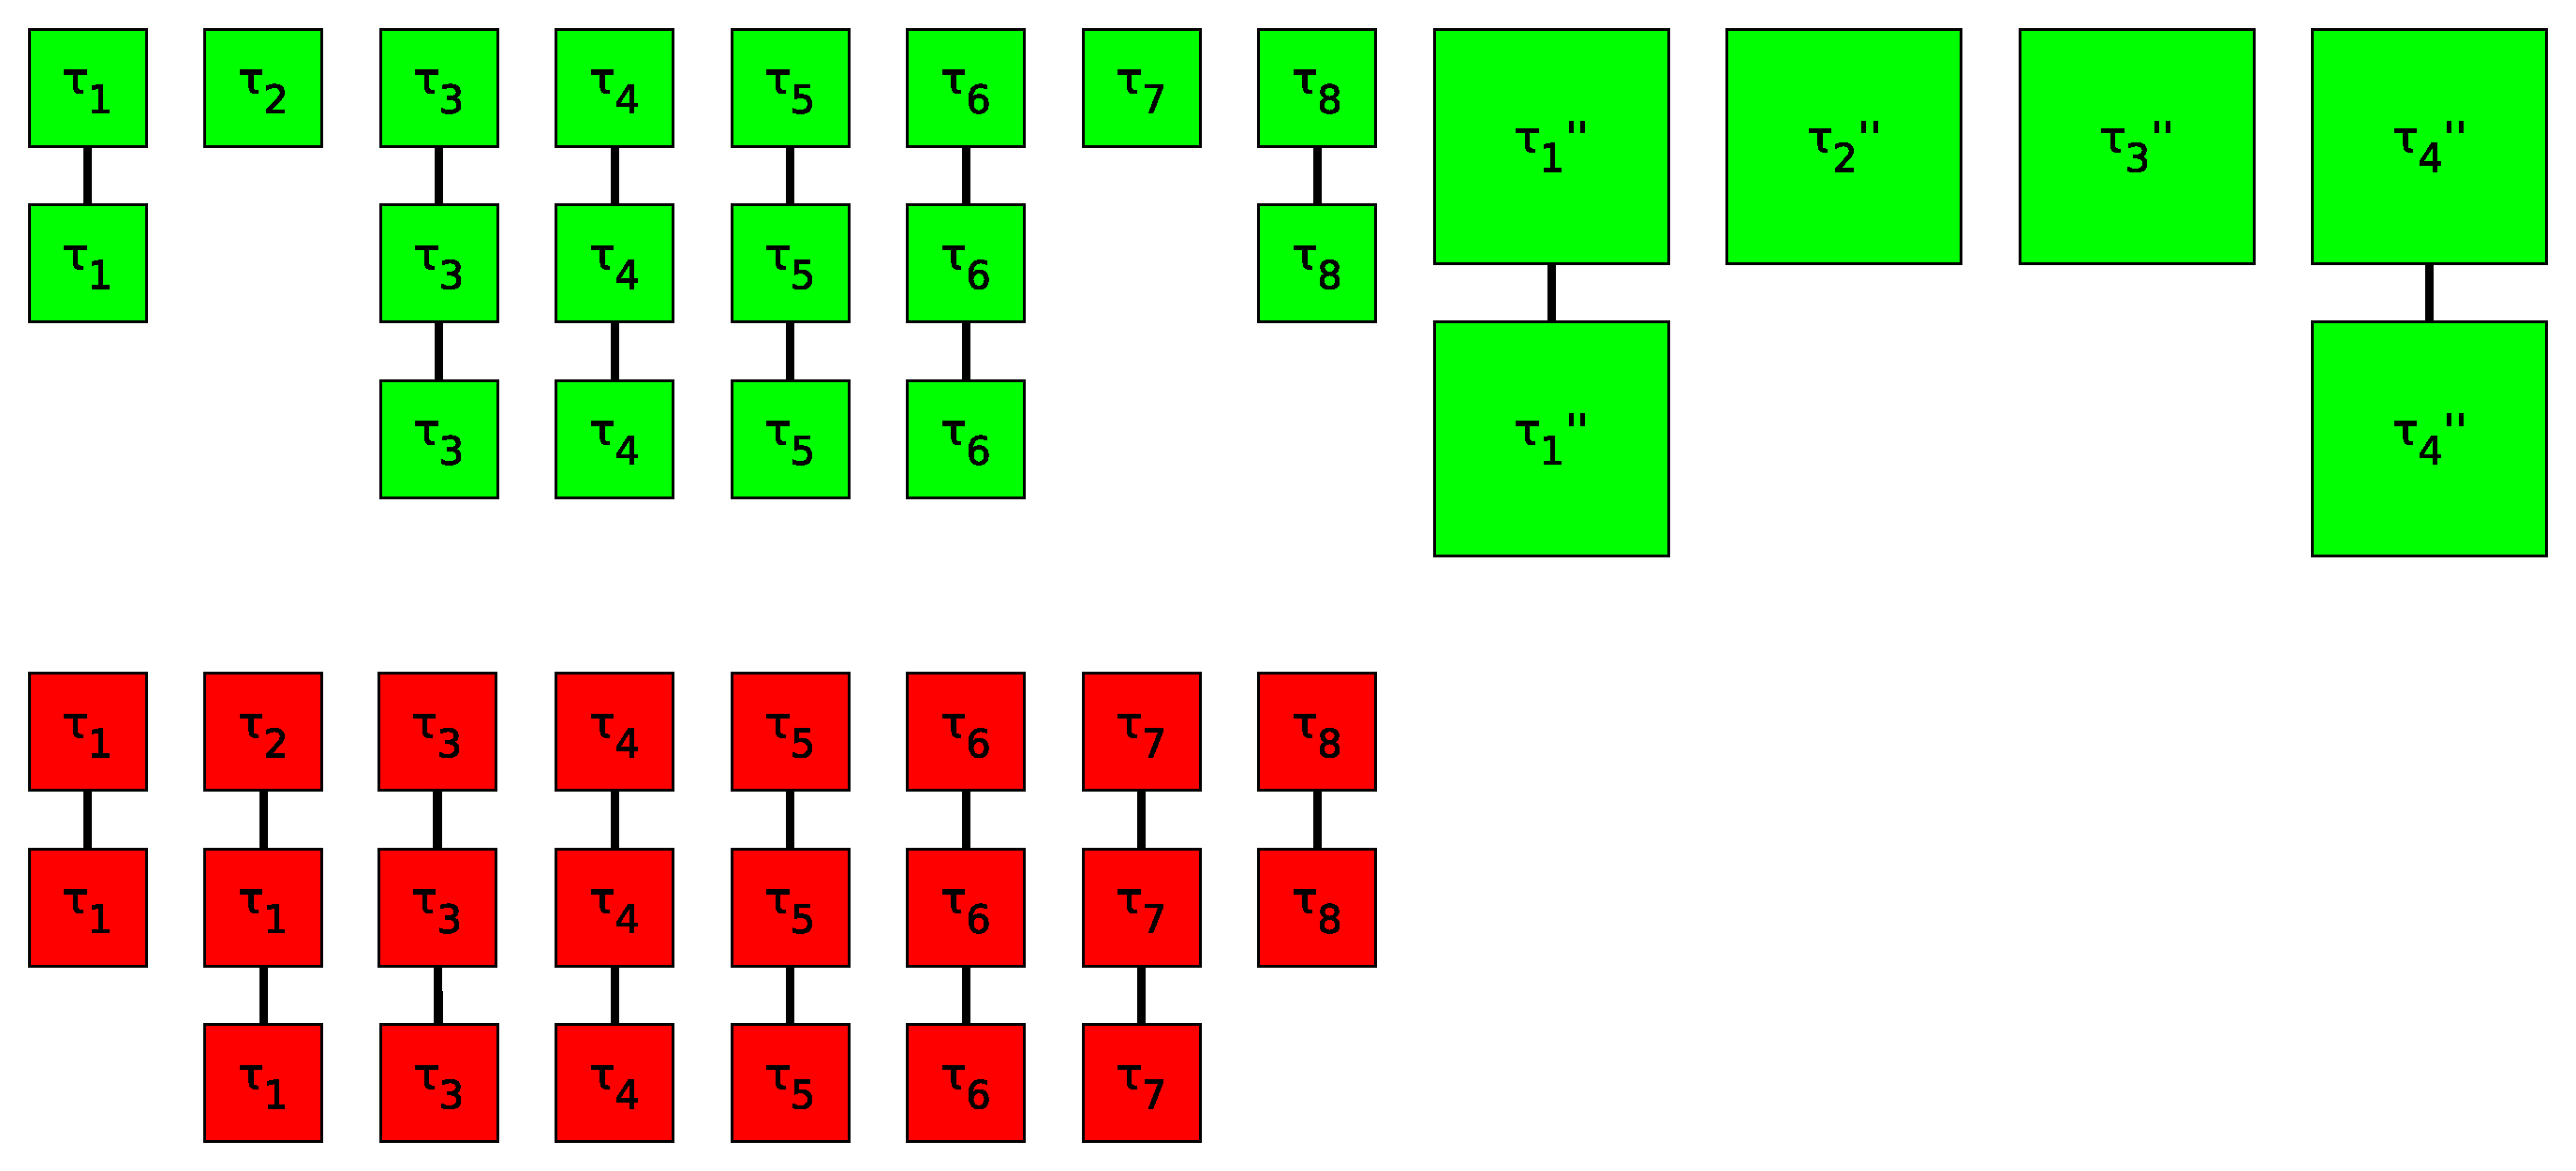
\includegraphics[width=\linewidth]{figures/fg-h2-matrix-block-orderd.pdf}
        \caption{Gruppierung von Blockmatrizen nach Fern- bzw. Nahfeld und nach
                 zuständigen Zeilencluster}
    \end{overprint}
  \end{figure}
\end{frame}

\begin{frame}{1. Phase (Fernfeld)}
  \begin{figure}
    \begin{overprint}
      \onslide<1>
        \centering
        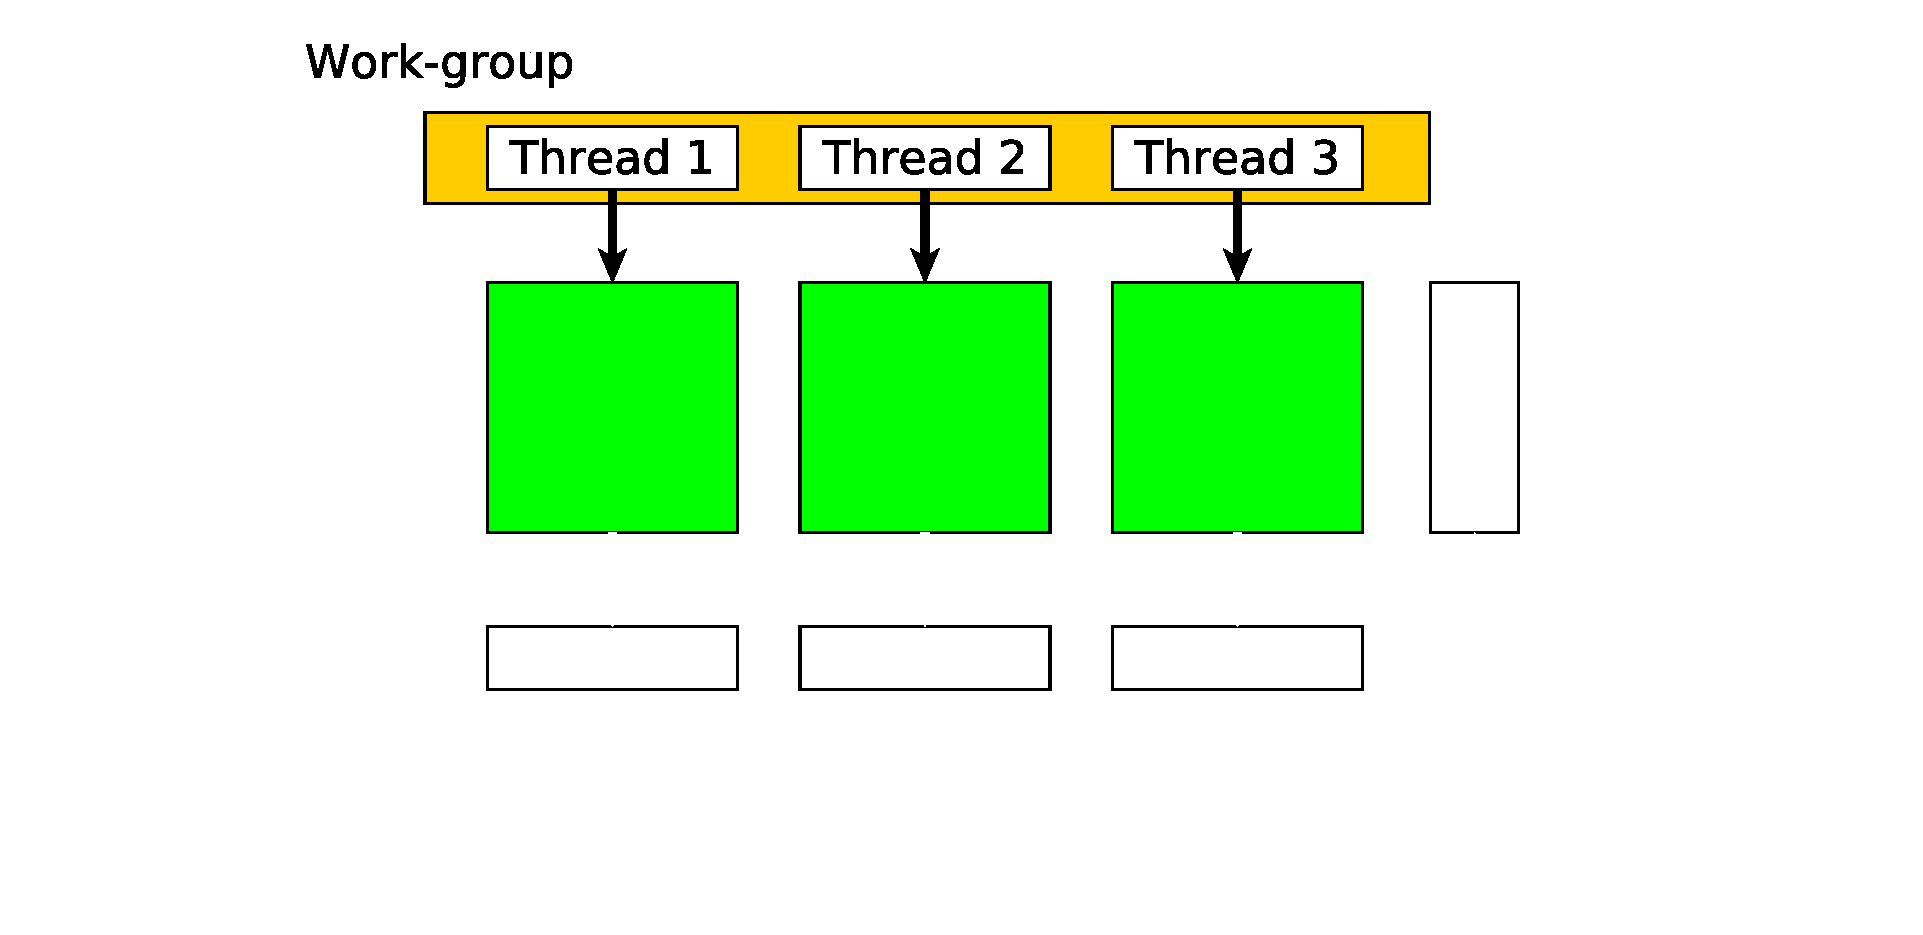
\includegraphics[width=\linewidth]{figures/fg-ff-initial-situation.pdf}
        \caption{Ausgangssituation einer Opencl work-group in der 1. Phase.}
      \onslide<2>
        \centering
        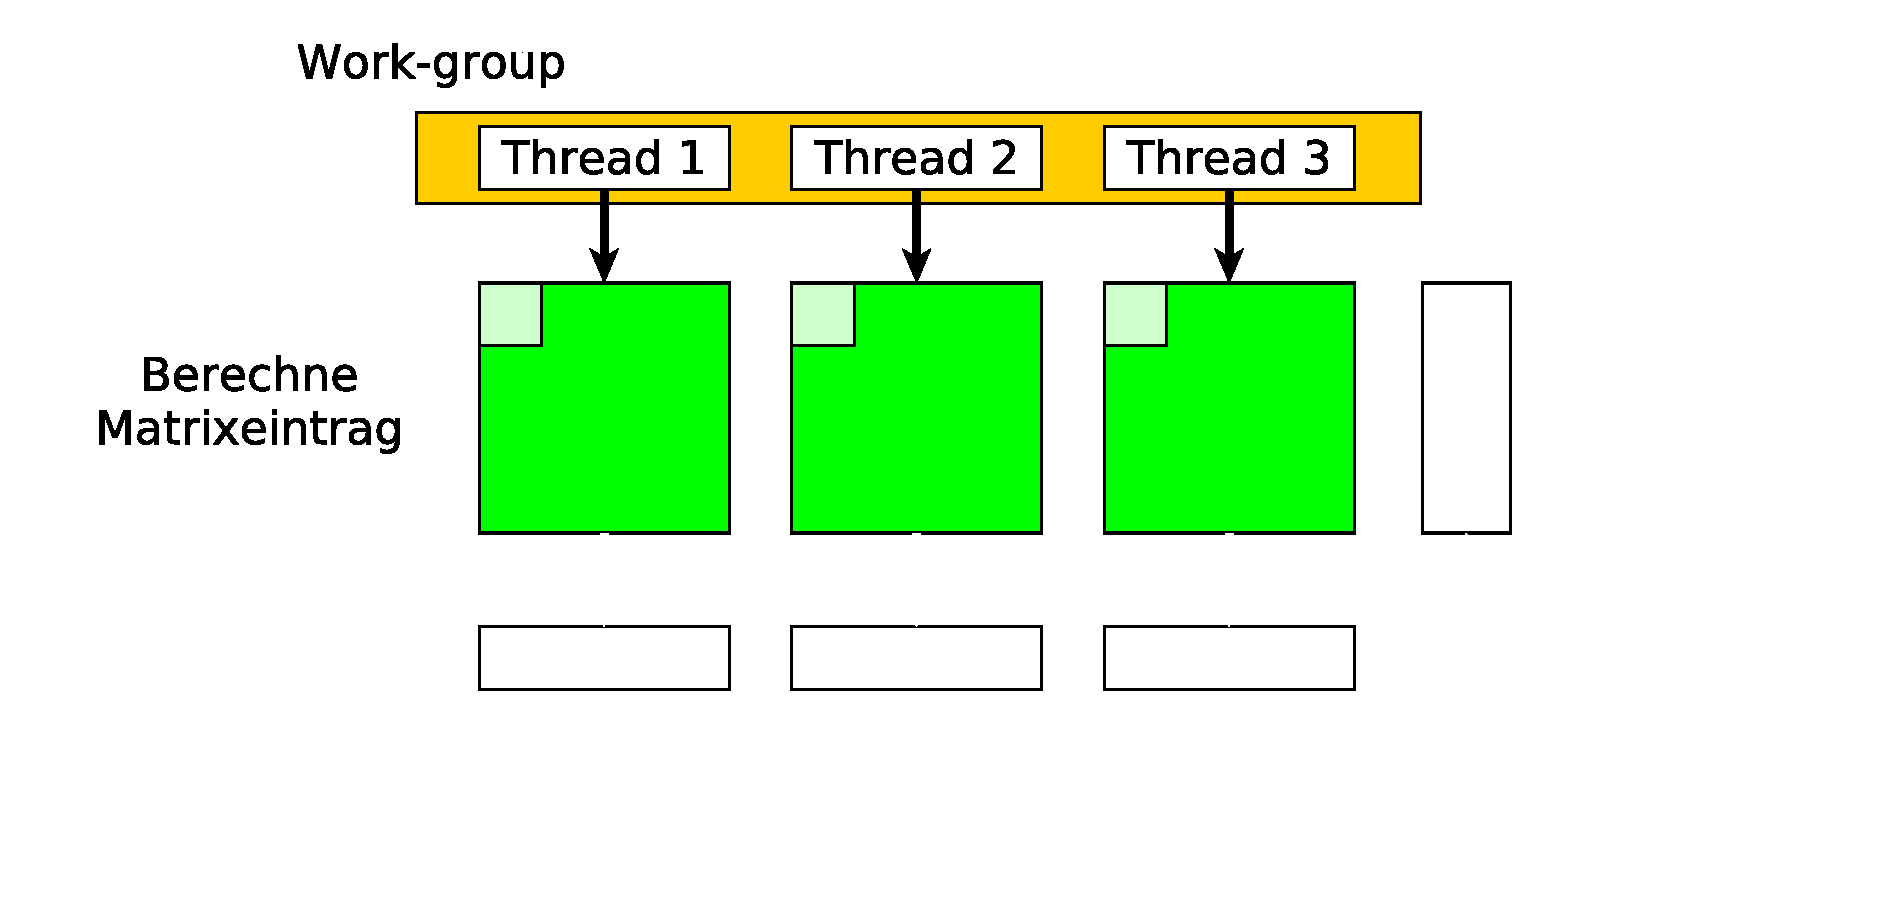
\includegraphics[width=\linewidth]{figures/fg-ff-compute-matrix-entry.pdf}
        \caption{Berechne den ersten Eintrag einer Matrixzeile.}
      \onslide<3>
        \centering
        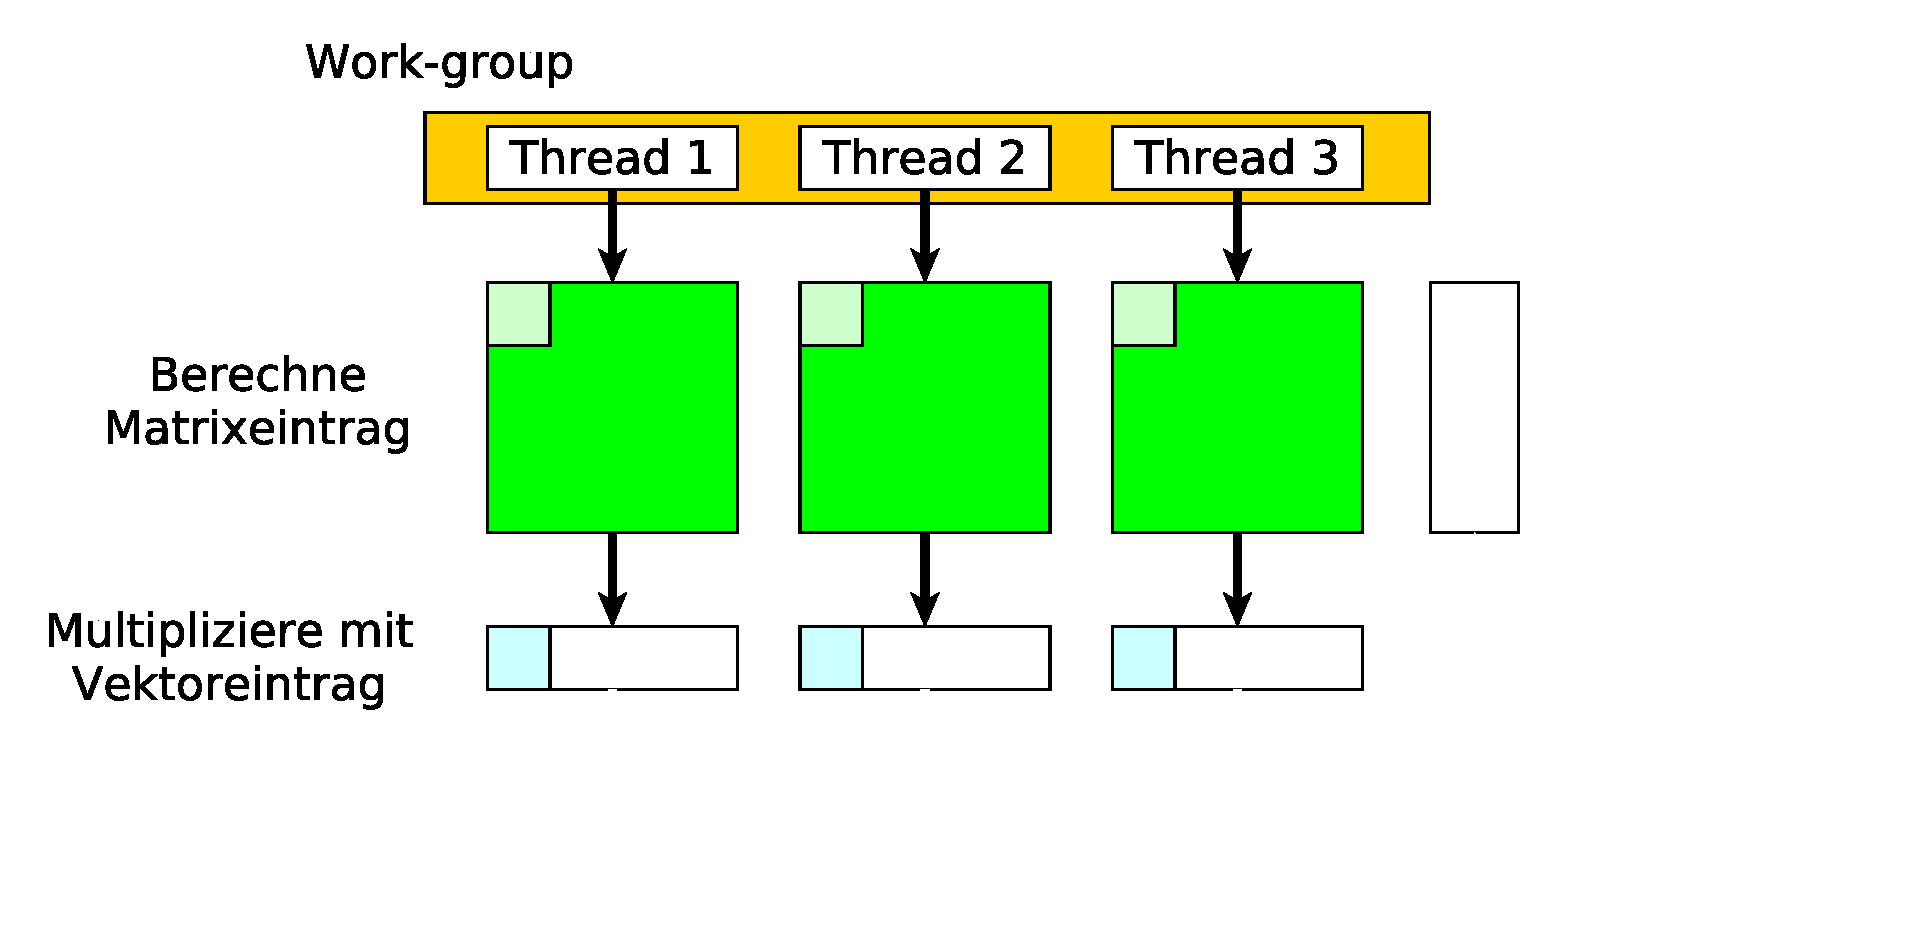
\includegraphics[width=\linewidth]{figures/fg-ff-multiply-vector.pdf}
        \caption{Multipliziere den Matrixeintrag mit dem entsprechenden Eintrag
                 des Eingabevektors.}
      \onslide<4>
        \centering
        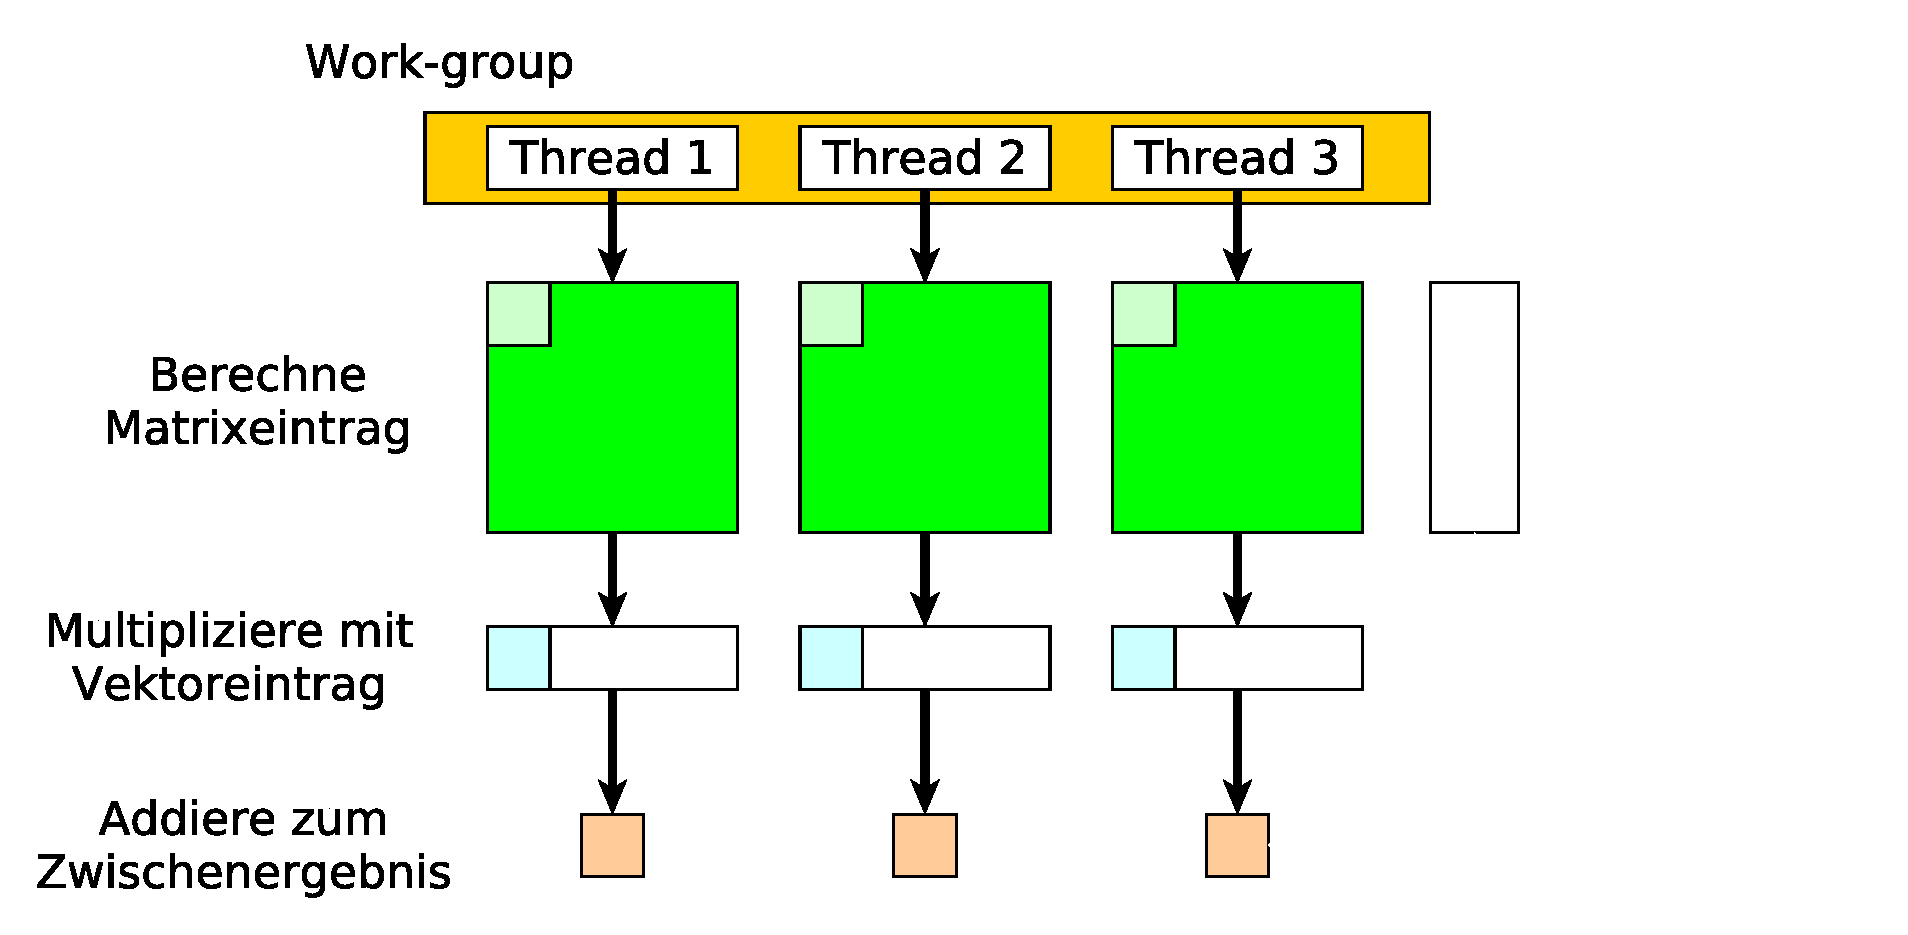
\includegraphics[width=\linewidth]{figures/fg-ff-add-interim-result.pdf}
        \caption{Addiere das Produkt zum Zwischenergebnis hinzu.}
      \onslide<5>
        \centering
        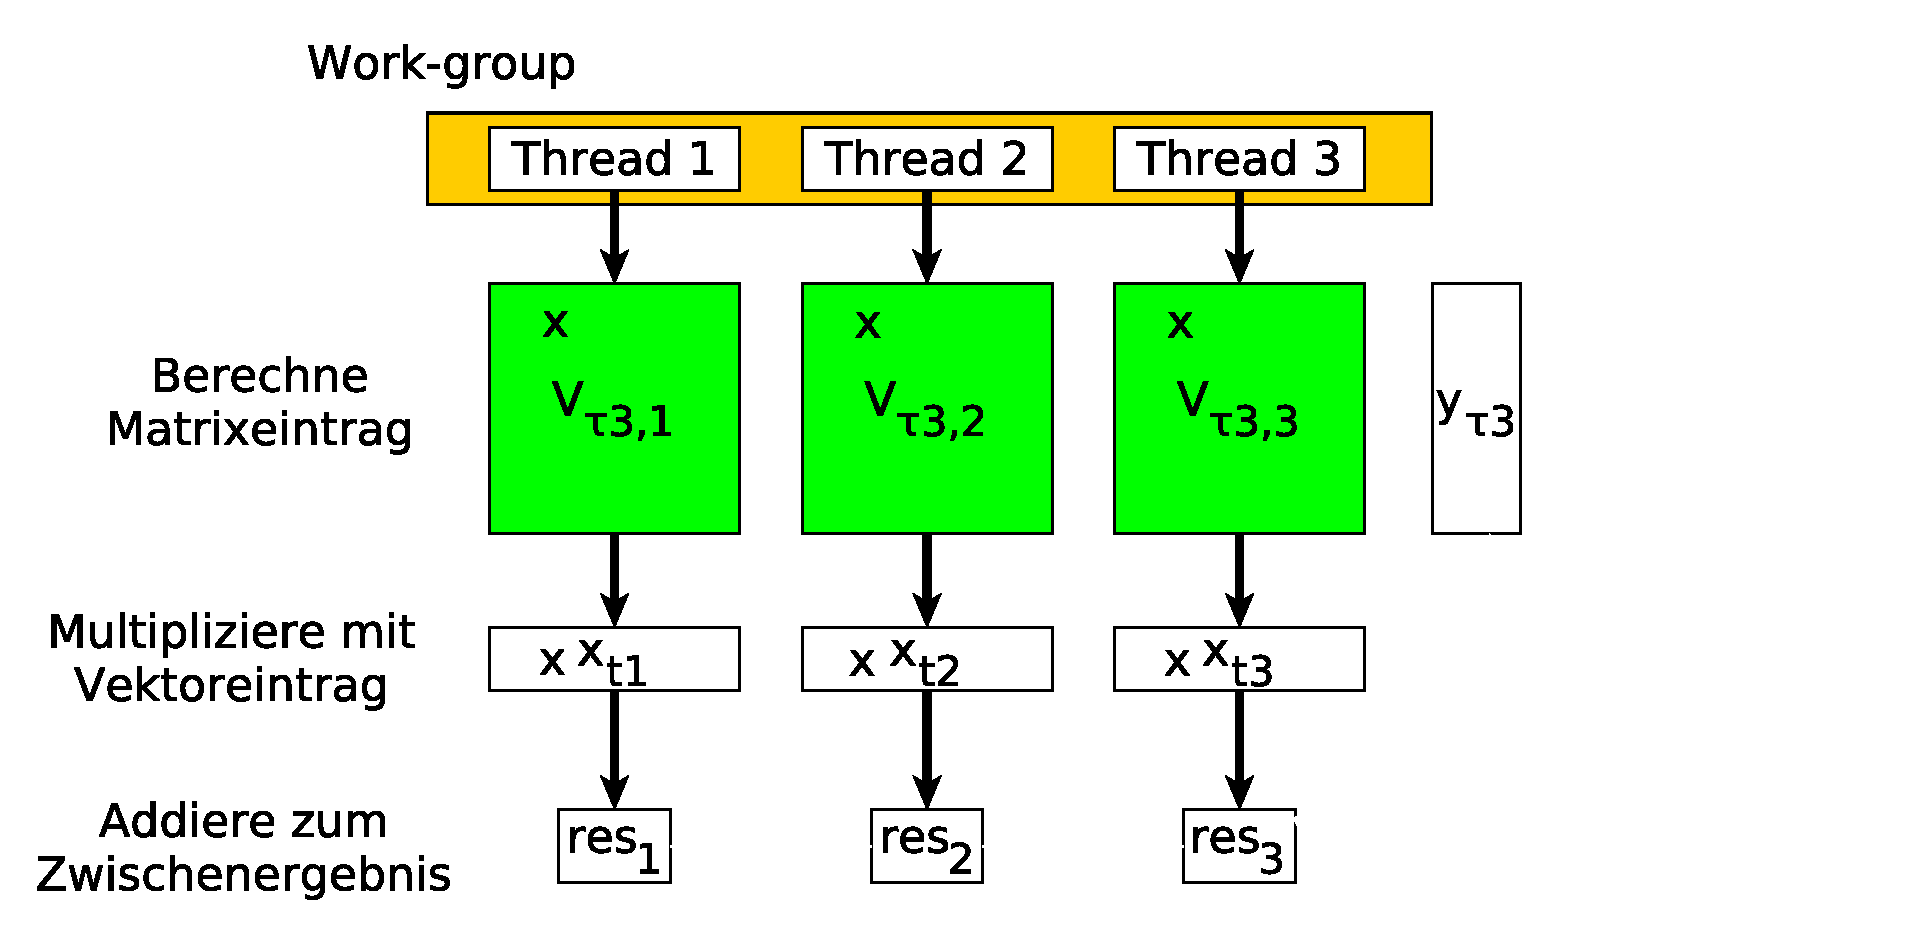
\includegraphics[width=\linewidth]{figures/fg-ff-next-column.pdf}
        \caption{Wiederhole die Prozedur für alle Einträge einer Zeile.}
      \onslide<6>
        \centering
        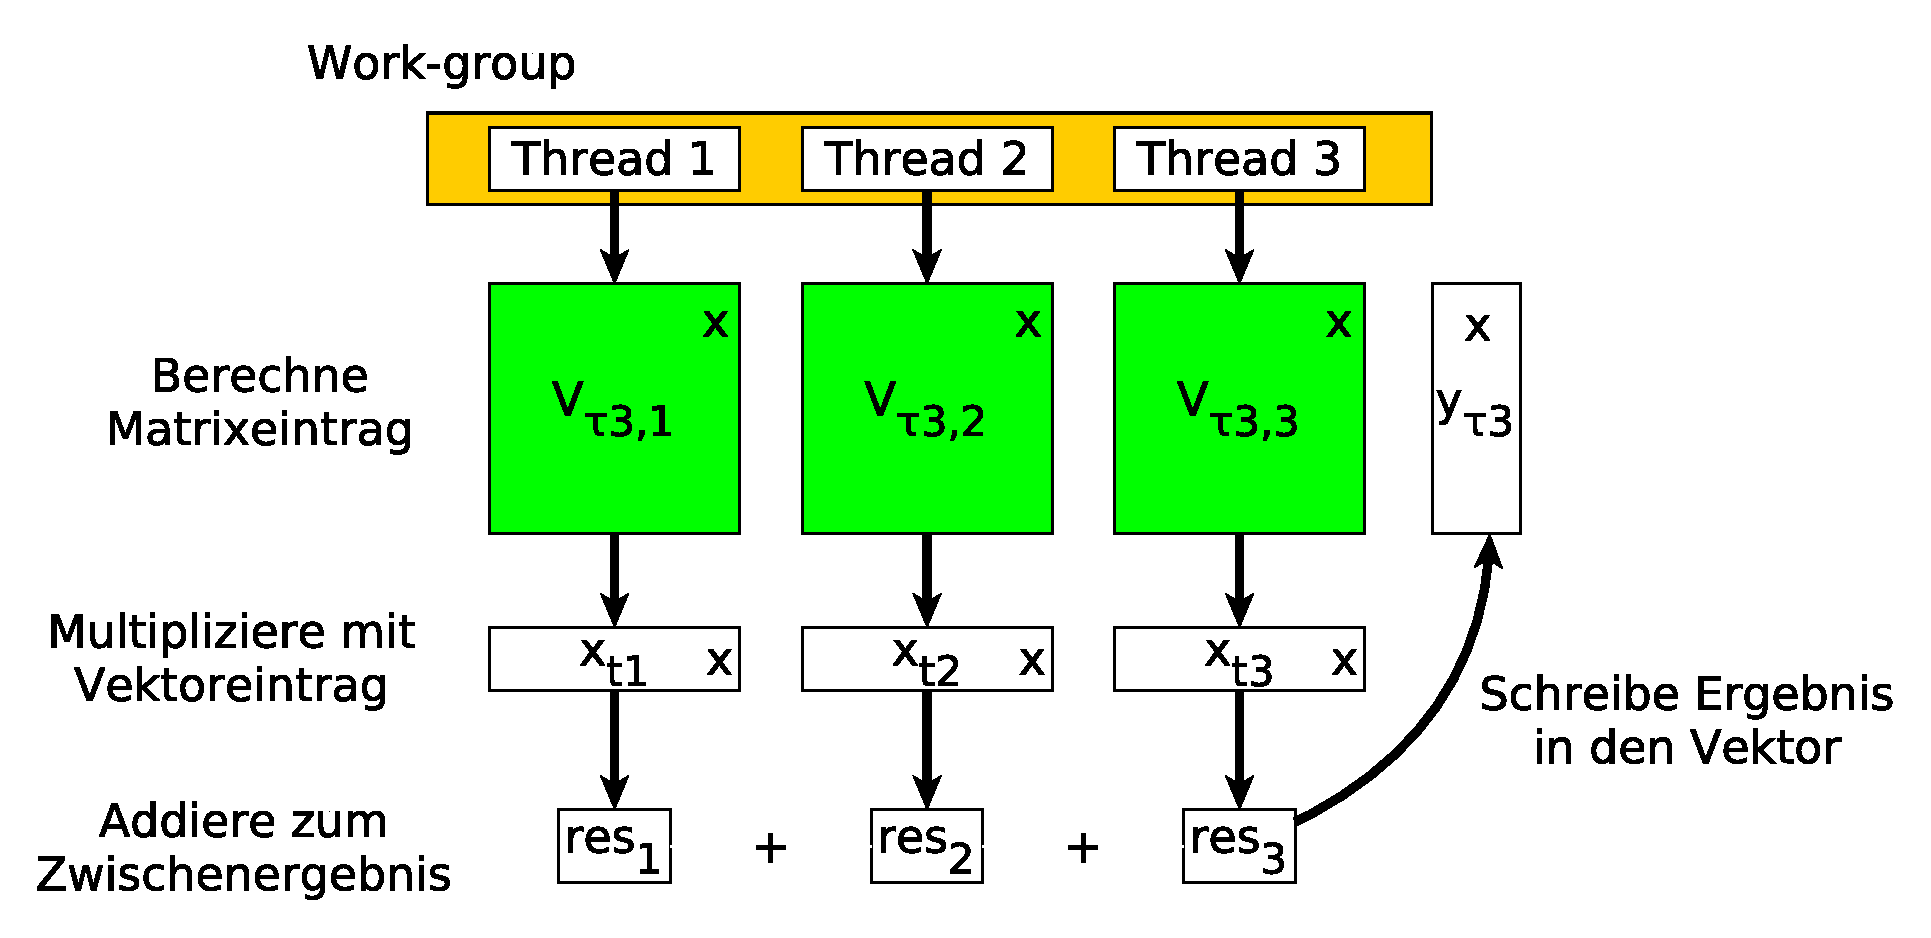
\includegraphics[width=\linewidth]{figures/fg-ff-write-result.pdf}
        \caption{Die Summe der Zwischenergebnisse ergiebt den Eintrag im
                 Ausgabevektor.}
    \end{overprint}
  \end{figure}
\end{frame}

\begin{frame}{1. Phase (Fernfeld)}
  \begin{figure}
    \centering
    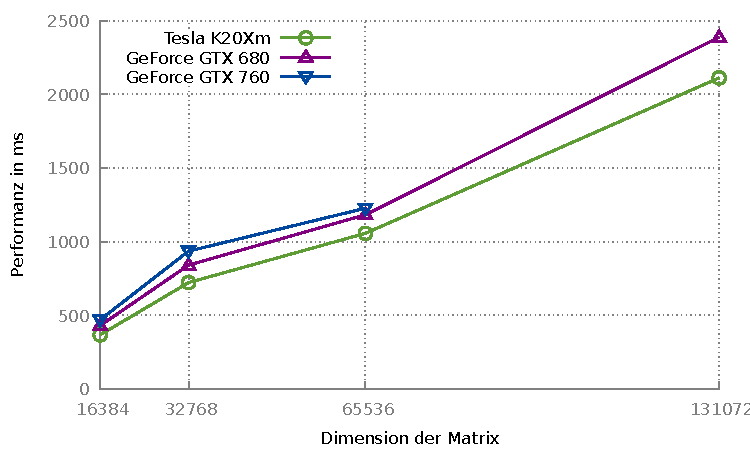
\includegraphics[width=\linewidth]{figures/fg-performance-ff.pdf}
    \caption{Performanz der 1.Phase auf verschiedenen GPUs.}
  \end{figure}
\end{frame}

\begin{frame}{1. Phase (Fernfeld)}
  \small
  \begin{table}
    \begin{tabular}{rrrrrr} \toprule
      \multirow{3}{*}{Dimension} & \multicolumn{5}{c}{Preformanz in ms} \\ \cmidrule{2-6}
      & \multicolumn{2}{c}{CPUs} |& \multicolumn{3}{c}{GPUs} \\ \cmidrule{2-6}
      & \begin{tabular}{@{}c@{}}Xeon \\ E5-4640\end{tabular}
      & \begin{tabular}{@{}c@{}}Core \\ i7-3820\end{tabular}
      & \begin{tabular}{@{}c@{}}Tesla \\ K20Xm\end{tabular}
      & \begin{tabular}{@{}c@{}}GeForce \\ GTX 680\end{tabular}
      & \begin{tabular}{@{}c@{}}GeForce \\ GTX 760\end{tabular} \\ \cmidrule{1-6}
       16384 &  16830.000 &  76423.179 &  367.612 &  430.675 &  469.848 \\
       32768 &  36960.000 & 167487.521 &  721.806 &  840.885 &  935.754 \\
       65536 &  74710.000 & 337433.000 & 1056.583 & 1182.343 & 1226.704 \\
      131072 & 154540.000 & 700738.240 & 2110.852 & 2387.168 & --- \\
      \bottomrule
    \end{tabular}
  \end{table}
  \normalsize
\end{frame}

\begin{frame}{2.-4. Phase (Nahfeld)}
  \begin{itemize}
    \item Nahfeld besteht aus allen Integraltypen
    \item Interpertation als Integrale mit unterschiedlichen/unterschiedlich
          vielen Quadraturpunkten
    \item Vertices zweier Dreiecke müssen zueinander permutiert werden\footnotemark[1]
  \end{itemize}
  \footnotesize
  \footnotetext[1]{Quelle: Efficient automatic quadrature in 3-d galerkin bem.}
  \normalsize
\end{frame}

\begin{frame}{2.-4. Phase (Nahfeld)}
  \begin{tabular}{cccccc} \cmidrule[\heavyrulewidth]{1-5}
     & \multicolumn{4}{c}{Anzahl gemeinsamer Vertices} & \\ \cmidrule{2-5}
    \multirow{2}{*}{Anzahl Quadraturpunkte} & 0 & 1 & 2 & 3 & \\ \cmidrule{2-5}
     & k & l & m & m & \(\Leftarrow\) 2.-4. Phase\\
    \cmidrule[\heavyrulewidth]{1-5}
  \end{tabular}
  \begin{itemize}
    \item \(k, l, m \in \mathbb{N}, k < l < m\)
  \end{itemize}
\end{frame}

\begin{frame}{2.-4. Phase (Nahfeld)}
  \begin{tabular}{cccccc} \cmidrule[\heavyrulewidth]{1-5}
     & \multicolumn{4}{c}{Anzahl gemeinsamer Vertices} & \\ \cmidrule{2-5}
    \multirow{2}{*}{Anzahl Quadraturpunkte} & 0 & 1 & 2 & 3 & \\ \cmidrule{2-5}
     & k & k     & k         & k         & \(\Leftarrow\) 2. Phase \\
     &   & l - k & l - k     & l - k     & \(\Leftarrow\) 3. Phase \\
     &   &       & m - l - k & m - l - k & \(\Leftarrow\) 4. Phase \\
    \cmidrule[\heavyrulewidth]{1-5}
  \end{tabular}
  \begin{itemize}
    \item \(k, l, m \in \mathbb{N}, k < l < m\)
  \end{itemize}
\end{frame}

\begin{frame}{2. Phase}
  \begin{itemize}
    \item Ähnlich wie in der 1. Phase, bis auf dass
    \begin{itemize}
      \item für jeden Matrixeintrag entschieden werden muss, welche
            Quadraturpunkte zu wählen sind.
      \item für jeden Matrixeintrag die entsprechenden Dreiecksvertices
            zueinander permutiert werden müssen.
    \end{itemize}
  \end{itemize}
\end{frame}

\begin{frame}{2. Phase}
  \small
  \begin{table}
    \begin{tabular}{rrrrrr} \toprule
      \multirow{3}{*}{Dimension} & \multicolumn{5}{c}{Preformanz in ms} \\ \cmidrule{2-6}
      & \multicolumn{2}{c}{CPUs} |& \multicolumn{3}{c}{GPUs} \\ \cmidrule{2-6}
      & \begin{tabular}{@{}c@{}}Xeon \\ E5-4640\end{tabular}
      & \begin{tabular}{@{}c@{}}Core \\ i7-3820\end{tabular}
      & \begin{tabular}{@{}c@{}}Tesla \\ K20Xm\end{tabular}
      & \begin{tabular}{@{}c@{}}GeForce \\ GTX 680\end{tabular}
      & \begin{tabular}{@{}c@{}}GeForce \\ GTX 760\end{tabular} \\ \cmidrule{1-6}
       16384 &  900.000 &  4547.475 &  72.462 &  64.436 &  75.006 \\
       32768 & 1780.000 &  9167.462 & 138.161 & 125.223 & 147.785 \\
       65536 & 3550.000 & 18162.474 & 273.268 & 246.615 & 291.429\\
      131072 & 7070.000 & 36480.016 & 528.493 & 480.287 & --- \\
      \bottomrule
    \end{tabular}
  \end{table}
  \normalsize
\end{frame}

\begin{frame}{3.-4. Phase}
  \begin{columns}
    \column{0.425\linewidth}
      \begin{algorithm}[H]
        \begin{algorithmic}[1]
          \footnotesize
          {
          \State{sum = 0}
          \For{q = 0; q < nq; ++q}
            \State{sum += \(w_{q}\) * kernel\relax(\(x_{q}, y_{q}\))}
          \EndFor{}
          }
          \State{result += sum}
        \end{algorithmic}
      \end{algorithm}
    \column{0.6\linewidth}
      \begin{algorithm}[H]
        \begin{algorithmic}[1]
          \footnotesize
          {
          \State{lid = get\_local\_id\relax(0)}
          \State{lsize = get\_local\_size\relax(0)}
          \State{sum = 0}
          \For{q = 0; q < nq; q += lsize}
            \If{(q + lid) < nq}
              \State{\(sum_{lid}\) += \(w_{q + lid}\) * kernel\relax(\(x_{q + lid}, y_{q + lid}\))}
            \EndIf{}
          \EndFor{}
          }
          \State{result += \(\sum\limits_{i = 0}^{lsize} sum_{i}\)}
        \end{algorithmic}
      \end{algorithm}
  \end{columns}
  \begin{center}
    Pseudocode zum sequentiellen (links) und Thread-level vektorisierten
    (rechts) Auswerten einer Quadratur.
  \end{center}
\end{frame}

\begin{frame}{3. Phase}
  \begin{figure}
    \centering
    \caption{Performanz der 3.Phase.}
  \end{figure}
\end{frame}

\begin{frame}{4. Phase}
  \begin{figure}
    \centering
    \caption{Performanz der 4.Phase.}
  \end{figure}
\end{frame}

\begin{frame}{Vergleiche}

\end{frame}

\begin{frame}{Zusammenfassung}
  \begin{itemize}
    \item Wir können den Speicherbedarf einer \(\mathcal{H}^2\)-Matrix um
          75-90\% reduzieren
    \item Der Rechenaufwand für eine
  \end{itemize}
\end{frame}

\begin{frame}[allowframebreaks]{References}

  \bibliography{presentation}
  \bibliographystyle{abbrv}

\end{frame}

\end{document}
